\chapter{Results}
\label{ch_results}
%%%%%%%%%%%%%%%%%%%%%%%%%%%%%%%%%%%%%%%%%%%
%%%%%%%%%%%%%%%%%%%%%%%%%%%%%%%%%%%%%%%%%%%



\section{Module Evaluation}

\subsection{Carrier Waveform Generation Performance}

Figure \ref{fig:carrier_steady_state} shows the steady-state output of the carrier waveform generation module (blue trace) and the constant high logic level at the input (red trace). The frequency of the output waveform was calculated to be 40.2kHz.

\begin{figure}[H]
	\centering
	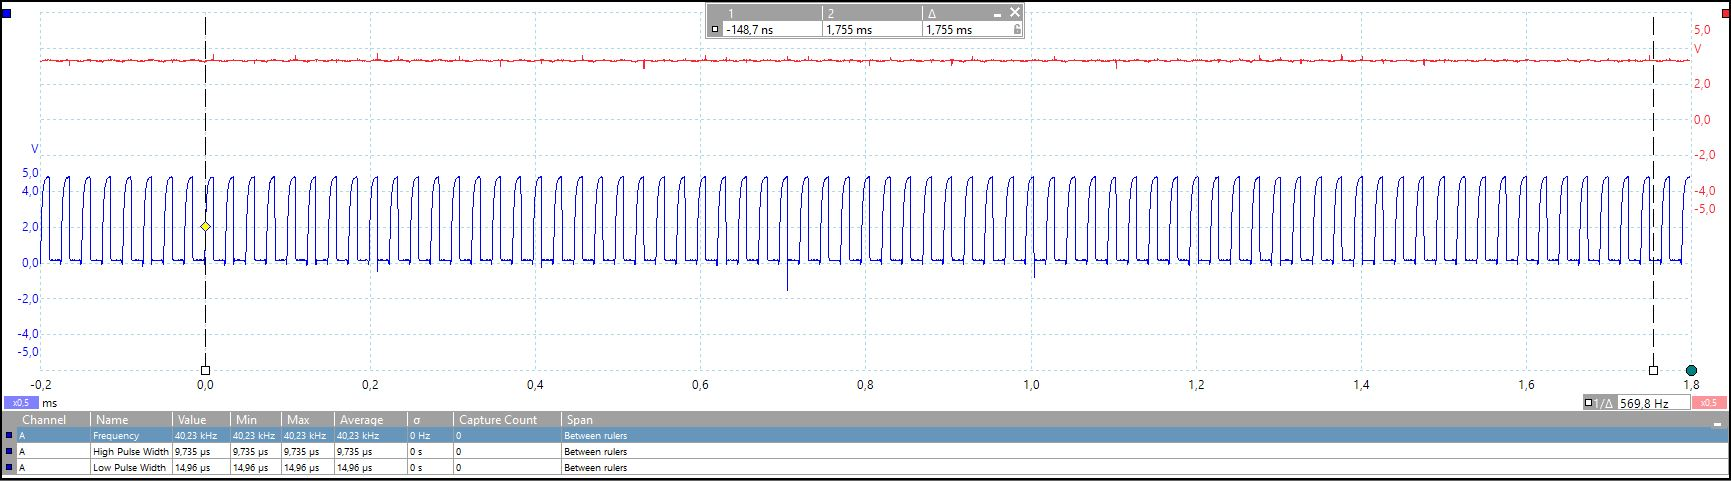
\includegraphics[width=.9\linewidth]{figures/results/carrier_waveform_generation/steady_state.JPG}
	\captionof{figure}{Carrier Generation - Constant Generation}
	\label{fig:carrier_steady_state}
\end{figure}

Figure \ref{fig:carrier_manchester_zoomed_view} presents a zoomed-in view of a Manchester transmission (red trace) at the input of the carrier waveform generation module and the corresponding output waveform (blue trace). The frequency of the carrier generated in these short bursts was measured to be 38.4kHz.

\begin{figure}[H]
	\centering
	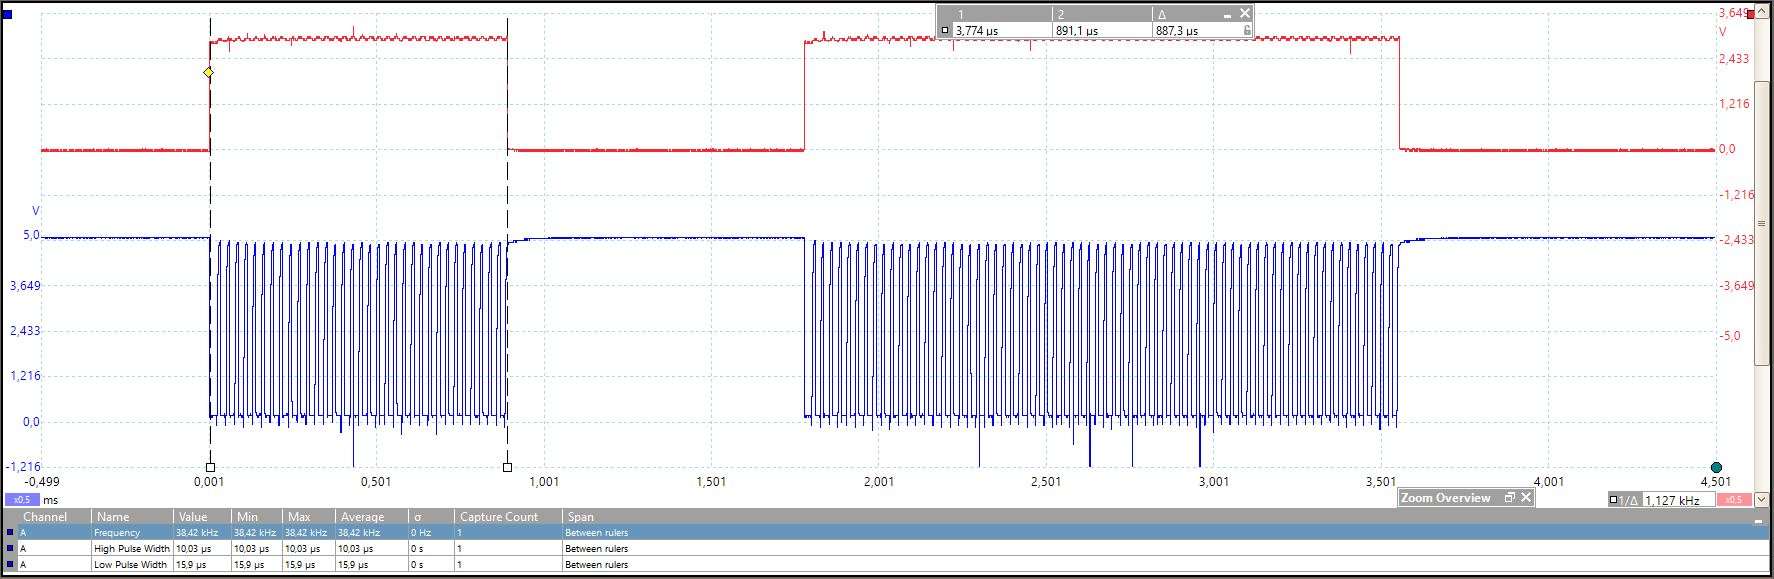
\includegraphics[width=.9\linewidth]{figures/results/carrier_waveform_generation/manchester_zoomed_view.JPG}
	\captionof{figure}{Manchester Transmission - Carrier Inspection}
	\label{fig:carrier_manchester_zoomed_view}
\end{figure}

In both cases, the duty cycle of the carrier waveform was 39\%.


%%%%%%%%%%	DISCUSSION	%%%%%%%%%%
\textbf{Discussion}\\
The 1.8kHz difference in tone frequency under different modes of operation might be as a consequence of the IC heating up during operation. It was observed that the temperature of the IC increased during prolonged operation.

The measured duty cycle is 6\% less than theoretically predicted, this difference is likely a consequence of the resistor tolerances, as the duty cycle depends only on the external resistors.

The duty cycle remaining the same for both modes of operation supports the hypothesis that the difference in frequency is due to an internal factor such as temperature.
%%%%%%%%%%	/DISCUSSION	%%%%%%%%%%


%%%%%%%%%%%%%%%%%%%%%%%%%%%%%%%%%%%%%%%%%%%




\subsection{Power LED Driver Performance}

The following screenshots shown in figures \ref{fig:pwr_led_6k} through \ref{fig:pwr_led_96k} show the results captured by the oscilloscope. The red trace shows the output of the function generator and the blue trace shows the voltage across the shunt resistor R1\footnote{see schematic in figure \ref{fig:schematic_power_led_driver}}.

\begin{figure}[H]
	\centering
	\begin{minipage}{.399\linewidth}
		\centering
		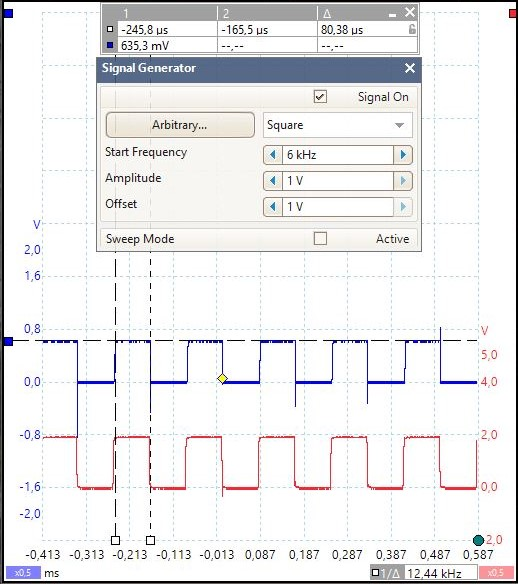
\includegraphics[width=\textwidth]{figures/results/power_led_driver/6khz_crop.JPG}
		\captionof{figure}{6kHz Driving Frequency}
		\label{fig:pwr_led_6k}
	\end{minipage}%
	\hspace{.1\linewidth}
	\begin{minipage}{.399\linewidth}
		\centering
		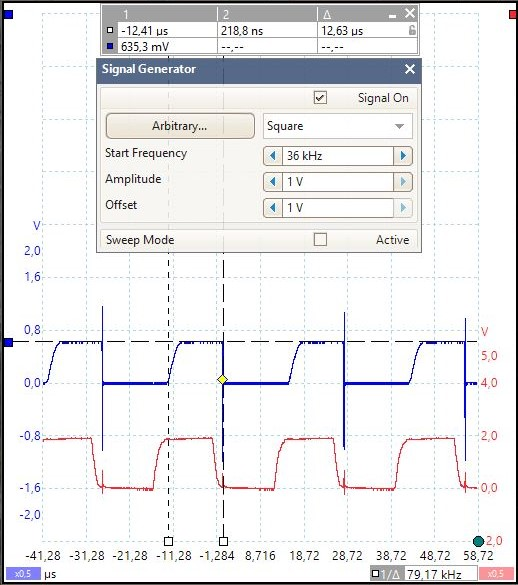
\includegraphics[width=\textwidth]{figures/results/power_led_driver/36khz_crop.JPG}
		\captionof{figure}{36kHz Driving Frequency}
		\label{fig:pwr_led_36k}
	\end{minipage}
\end{figure}

\begin{figure}[H]
	\centering
	\begin{minipage}{.4\linewidth}
		\centering
		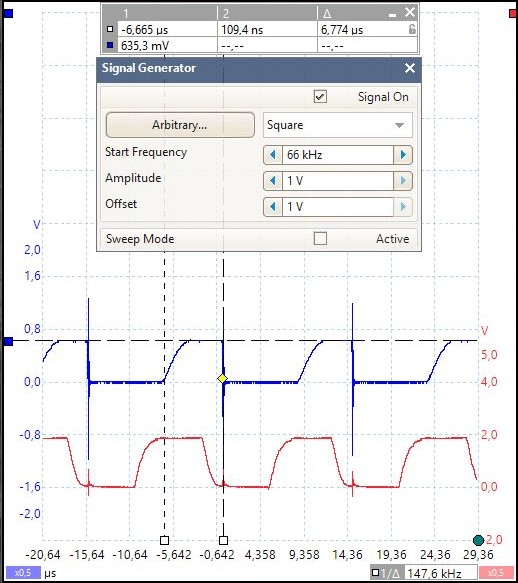
\includegraphics[width=\textwidth]{figures/results/power_led_driver/66khz_crop.JPG}
		\captionof{figure}{66kHz Driving Frequency}
		\label{fig:pwr_led_66k}
	\end{minipage}
	\hspace{.1\linewidth}
	\begin{minipage}{.4\linewidth}
		\centering
		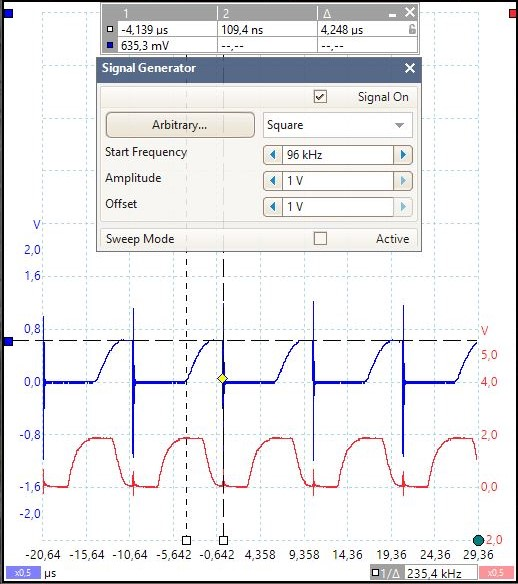
\includegraphics[width=\textwidth]{figures/results/power_led_driver/96khz_crop.JPG}
		\captionof{figure}{96kHz Driving Frequency}
		\label{fig:pwr_led_96k}
	\end{minipage}
\end{figure}

\begin{table}[H]
	\centering
	\begin{tabular}{ccc}
		\hline
		\textbf{\begin{tabular}[c]{@{}c@{}}Frequency\\ (kHz)\end{tabular}} & \textbf{\begin{tabular}[c]{@{}c@{}}LED Current\\ (mA)\end{tabular}} & \textbf{\begin{tabular}[c]{@{}c@{}}Duty Cycle\\ (\%)\end{tabular}} \\ \hline
		6 & 908 & 48.2 \\ \hline
		36 & 908 & 45.5 \\ \hline
		66 & 908 & 44.7 \\ \hline
		96 & 908 & 40.8 \\ \hline
	\end{tabular}
	\caption{Frequency V.S. Current and Pulse Width}
	\label{tbl:led_driver_tabulated_results}
\end{table}


%%%%%%%%%%	DISCUSSION	%%%%%%%%%%
\textbf{Discussion}\\
For each test frequency, the power LED driver module regulated the current with high precision and no noticeable ripple. This encapsulates the advantages of linear regulation.

The design predicted a current limit of 1.02A. These results show that the actual current limit is 0.91A. This result predicts that the real base-emitter voltage drop\footnote{at equilibrium} is closer to 0.62V.

The duty cycle of the LED current decreases for increasing input frequencies. This can be attributed to the rise-time of the current through the LED (the time taken for the current to reach a steady-state). As the driving frequency increases, this rise-time makes up an increasing proportion of the total on-time.
%%%%%%%%%%	/DISCUSSION	%%%%%%%%%%


%%%%%%%%%%%%%%%%%%%%%%%%%%%%%%%%%%%%%%%%%%%





\subsection{Light Focus System}

\subsubsection{Focal Length of Lens}

The focal length of the lens was measured to be 53mm. Figure \ref{fig:focal_length_experiemnt_result} shows the point formed after positioning the lens to one focal length above the working surface.

\begin{figure}[H]
	\centering
	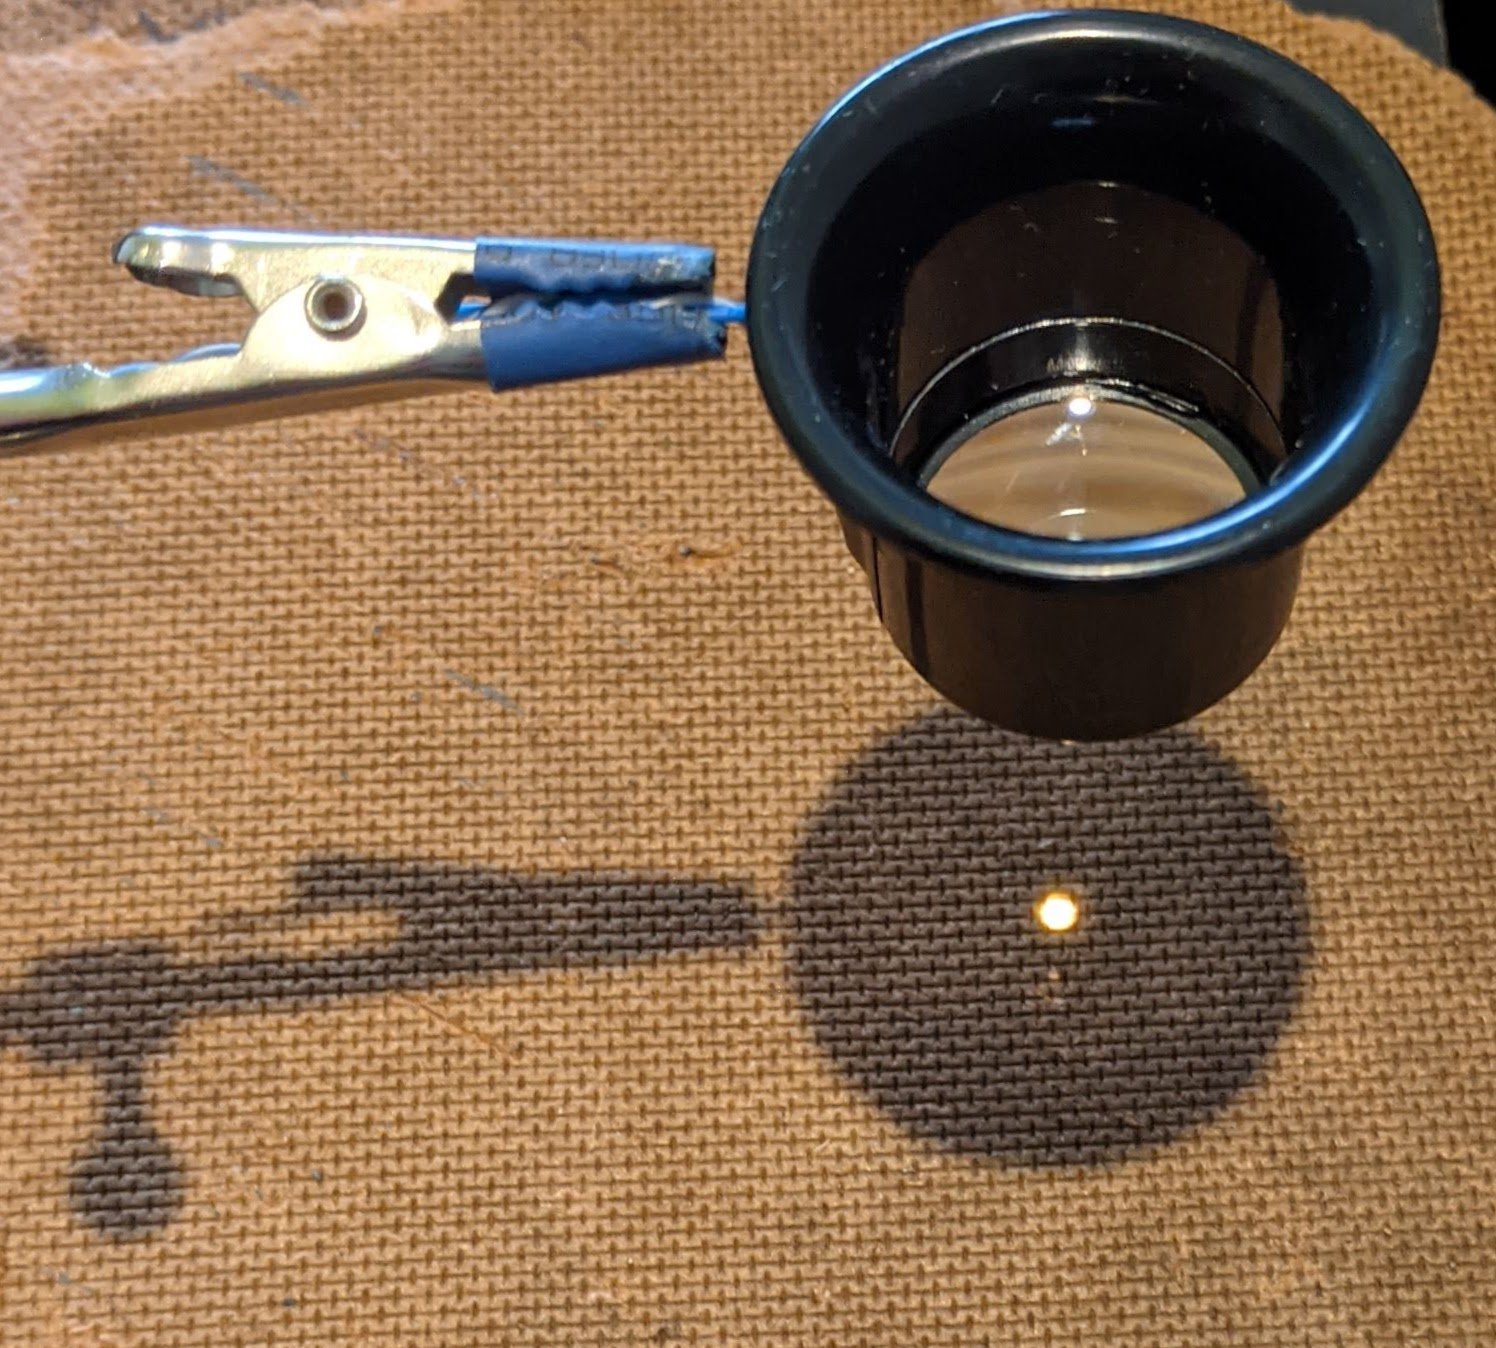
\includegraphics[width=.6\linewidth]{figures/results/focal_length_result.jpg}
	\captionof{figure}{Focal Length Experiemnt}
	\label{fig:focal_length_experiemnt_result}
\end{figure}


\subsubsection{IR Beam Dispersion}

\begin{figure}[H]
	\centering
	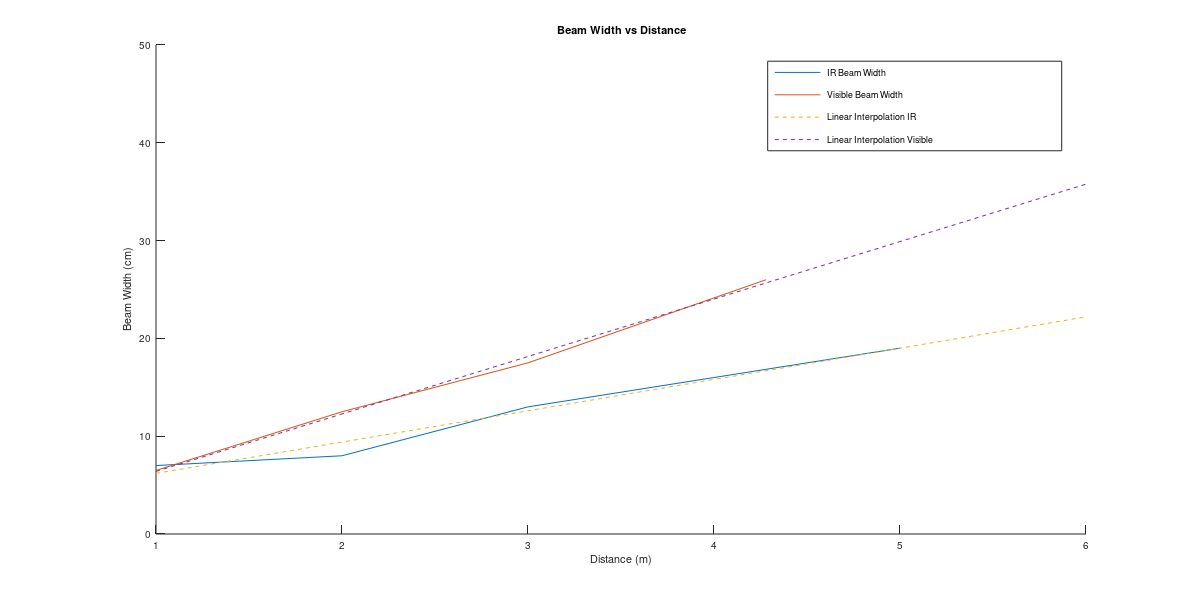
\includegraphics[width=\linewidth]{figures/results/beam_width_vs_distance.png}
	\captionof{figure}{Beam Width vs Distance}
	\label{fig:beam_width_vs_distance}
\end{figure}



Table \ref{tbl:spot_size_vs_distance} below shows the beam spot size vs distance for the IR and visible light power LEDs.

\begin{figure}[H]
	\centering
	\begin{minipage}{.4\textwidth}
		\textbf{Linear Interpolation Equations}
		
		\[width_{ir\: beam} = 0.03 + 0.032 \times d_{beam}\]
		
		\[width_{visible\: beam} = 0.00526 + 0.0587 \times d_{beam}\]
		
		
	\end{minipage}%
	\hspace{.1\textwidth}
	\begin{minipage}{.4\textwidth}
		\begin{table}[H]
			\begin{tabular}{ccc}
				\hline
				\textbf{\begin{tabular}[c]{@{}c@{}}Distance\\ (m)\end{tabular}} & \textbf{\begin{tabular}[c]{@{}c@{}}IR Beam\\ Width\\ (cm)\end{tabular}} & \textbf{\begin{tabular}[c]{@{}c@{}}Visible Beam\\ Width\\ (cm)\end{tabular}} \\ \hline
				1 & 7 & 6.5 \\ \hline
				2 & 8 & 12.5 \\ \hline
				3 & 13 & 17.5 \\ \hline
				4 & 16 & - \\ \hline
				4.28 & - & 26 \\ \hline
				5 & 19 & - \\ \hline
			\end{tabular}
			\captionof{table}{Tabulation of Spot Diameter V.S. Distance}
			\label{tbl:spot_size_vs_distance}
		\end{table}
	\end{minipage}
\end{figure}

%%%%%%%%%%	DISCUSSION	%%%%%%%%%%
\textbf{Discussion}\\
The diameter of the beam of parallel light rays produced by the light focus system is 22mm as this is the diameter of the lens. This experiment reveals however that not all the light leaves the lens parallel to the normal. This is probably as a consequence of the LED's size relative to the lens and to a lesser extent as a result of imperfect positioning of the light relative to the lens.

The large discrepancy between the beam angles of the IR and visible light is possibly an artefact from using a camera to trace the edge of the IR beam sport. The camera converts the detected light into a digital representation which might explain the non-linearities in figure \ref{tbl:spot_size_vs_distance}.

It should be noted that no chromatic aberration was observed while testing with the visible light LED, this suggests that any effects arising from the slightly longer wavelength of IR\footnote{940nm wavelength} light were negligible.
%%%%%%%%%%	/DISCUSSION	%%%%%%%%%%


%%%%%%%%%%%%%%%%%%%%%%%%%%%%%%%%%%%%%%%%%%%




\subsection{Directivity of IR Modules}

Figure \ref{fig:vrms_vs_angle_of_incidence} shows the root mean square (RMS) voltage value of the module's output versus the angle of incidence. Figure \ref{fig:beam_pattern} shows the normalized RMS voltage value and mirrors the image about the vertical to illustrate the beam pattern.


\begin{figure}[H]
	\centering
	\begin{minipage}{.4\linewidth}
		\centering
		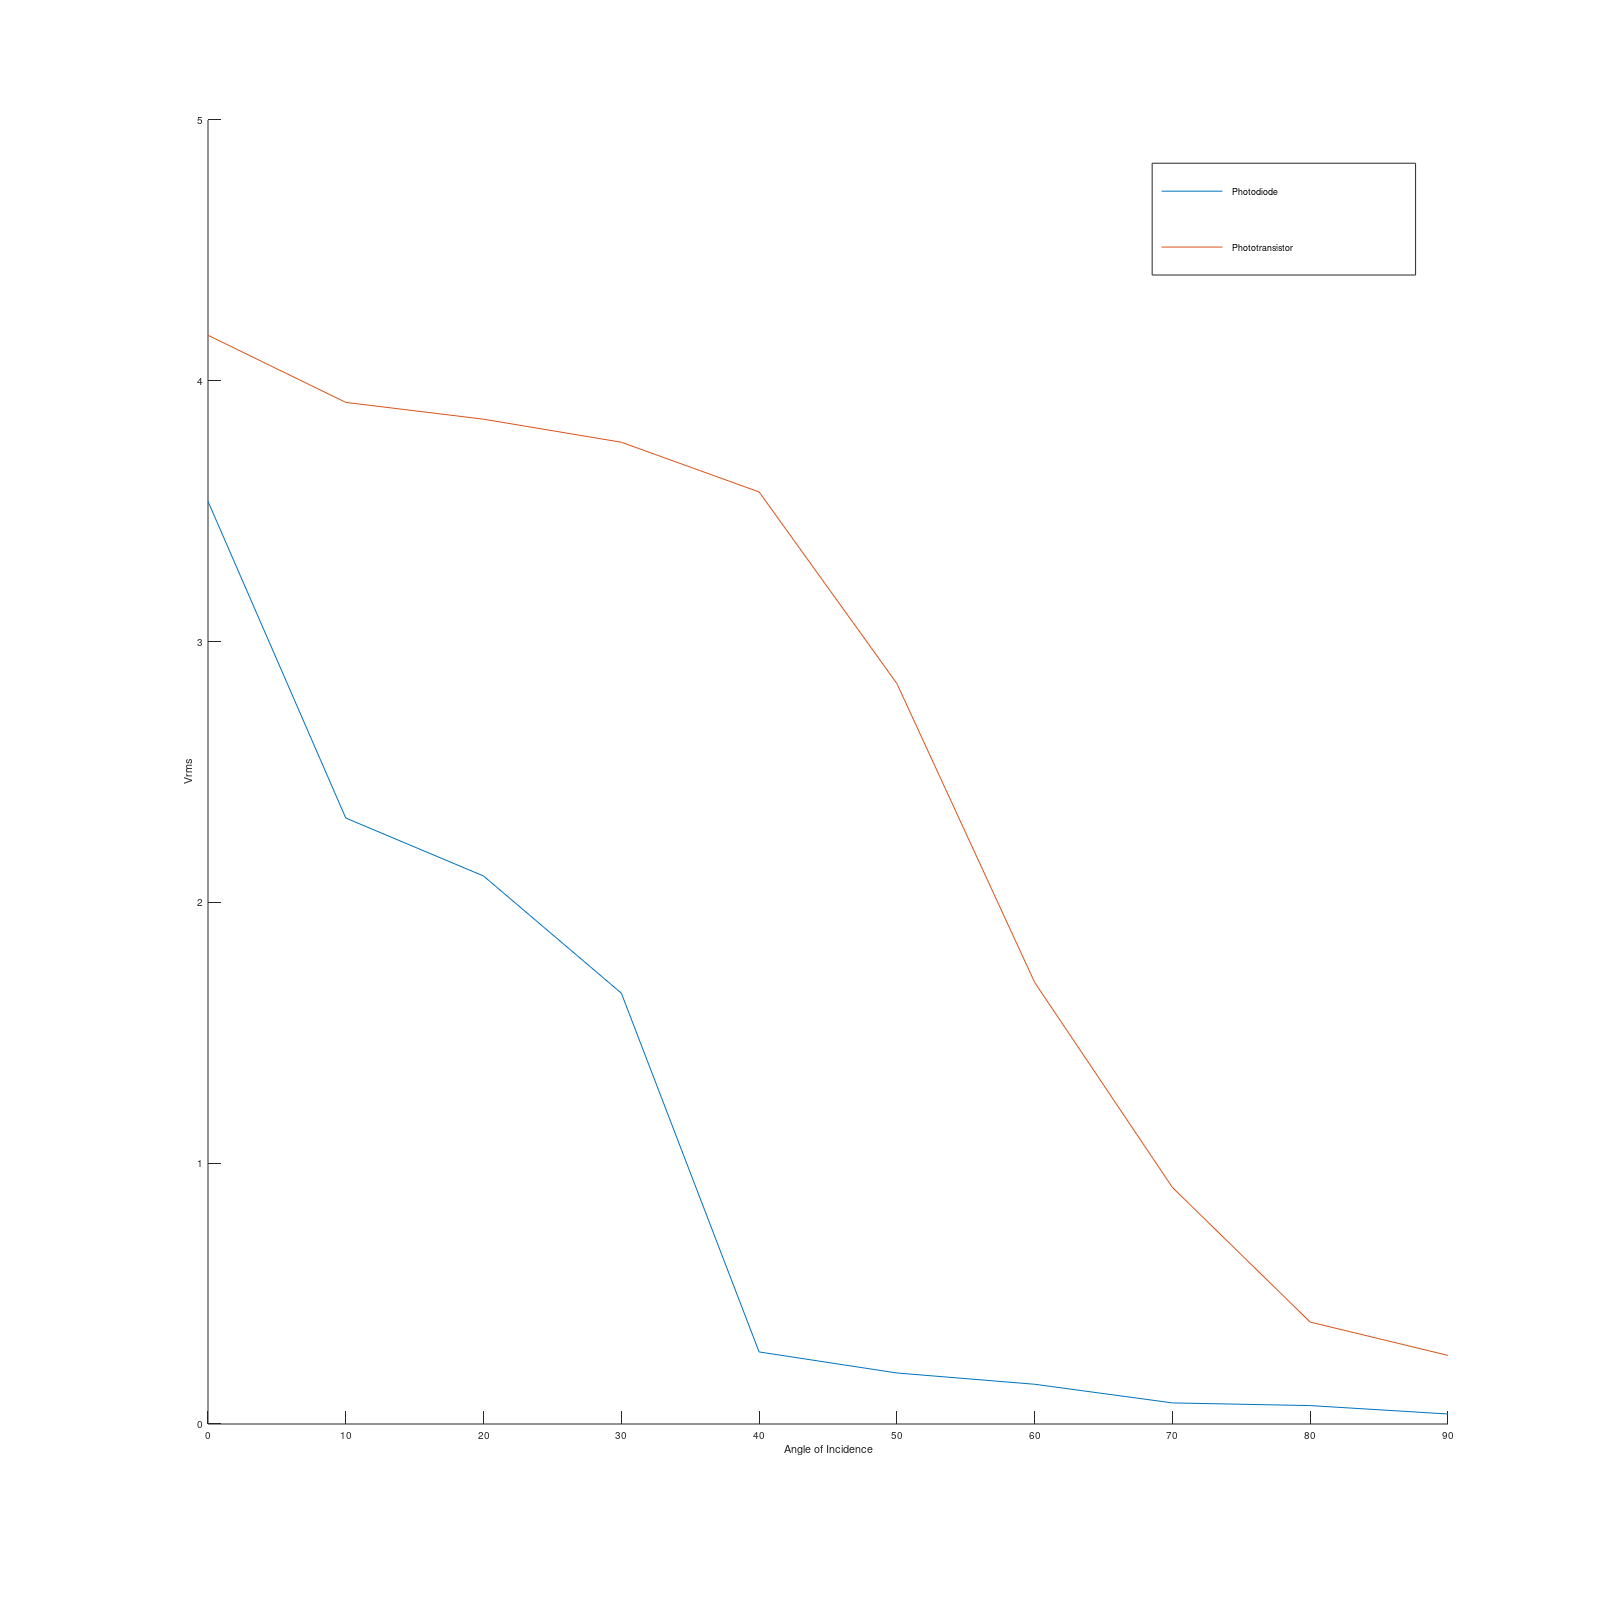
\includegraphics[width=\textwidth]{figures/results/vrms_vs_incidence_square.png}
		\captionof{figure}{Vrms vs Angle of Incidence}
		\label{fig:vrms_vs_angle_of_incidence}
	\end{minipage}
	\hspace{.1\linewidth}
	\begin{minipage}{.4\linewidth}
		\centering
		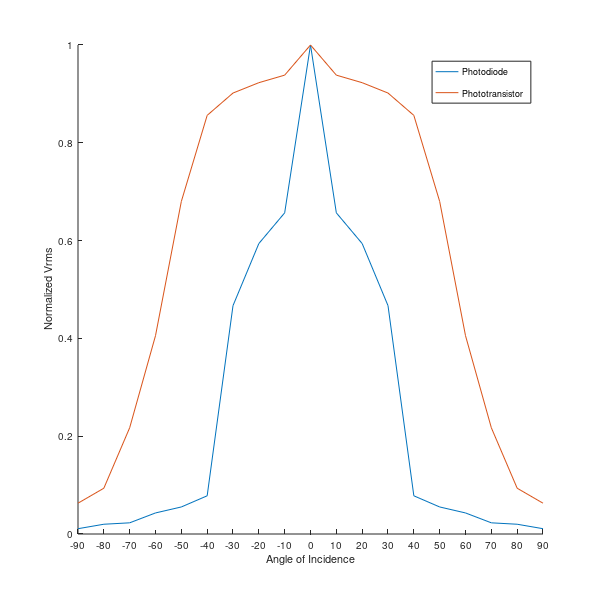
\includegraphics[width=\textwidth]{figures/results/beam_pattern_square.png}
		\captionof{figure}{Beam Pattern}
		\label{fig:beam_pattern}
	\end{minipage}
\end{figure}

The IR receiver module registered the signal between angles of 0\textdegree{} and 70\textdegree{} and failed to register a signal for angles greater than 80\textdegree. Between 70\textdegree{} and 80\textdegree{} the output would toggle sporadically.


%%%%%%%%%%	DISCUSSION	%%%%%%%%%%
\textbf{Discussion}\\
These results show that the phototransistor has the larger beam pattern, however, even with the larger beam pattern after an angle of 50\textdegree the sensitivity decreases rapidly.

These results do not simply quantify the limitations of the detector modules, they also provide the necessary information required to optimally orientate multiple sensors into arrays to obtain a large effective beam pattern.
%%%%%%%%%%	/DISCUSSION	%%%%%%%%%%




%%%%%%%%%%%%%%%%%%%%%%%%%%%%%%%%%%%%%%%%%%%




\subsection{Signal Conditioning Performance}

\subsubsection{Anti-alias Filtering}
Figure \ref{fig:anti_alias_filtering} below shows the oscilloscope trace of the 36kHz square waveform being generated at the input to the signal conditioning module (blue) and the filtered output waveform (red).

\begin{figure}[H]
	\centering
	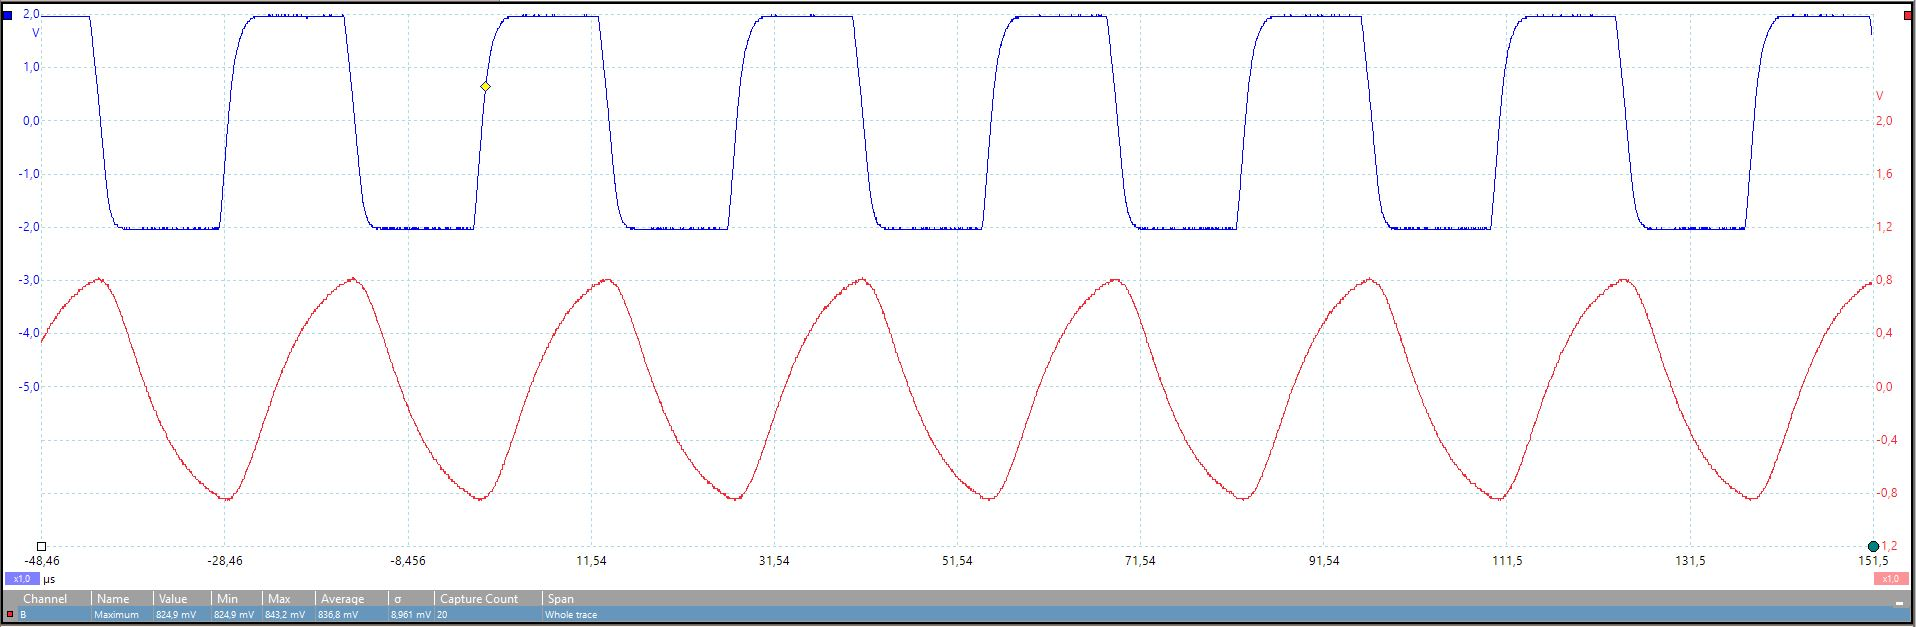
\includegraphics[width=\textwidth]{figures/results/low_pass_filter/36kHzsquarewavein.JPG}
	\captionof{figure}{Osciliscope output showing signal before and after filtering}
	\label{fig:anti_alias_filtering}
\end{figure}

%%%%%%%%%%	DISCUSSION	%%%%%%%%%%
%comment: this is lame but not much else to say...
\textbf{Discussion}\\
Visual inspection confirms that the anti-alias filter is removing the higher frequency components by virtue of the smoothed waveform at the output. The amplitude of the output waveform is less than half the amplitude of the input waveform, this reduction is mostly as a consequence of the voltage divider at the filter's input.
%%%%%%%%%%	/DISCUSSION	%%%%%%%%%%

\subsubsection{Precision Rectification}

Figure \ref{fig:precision_rectification} below shows the oscilloscope trace of the signal being fed into the precision rectifier (blue trace) and the resulting rectified signal (red trace).

\begin{figure}[H]
	\centering
	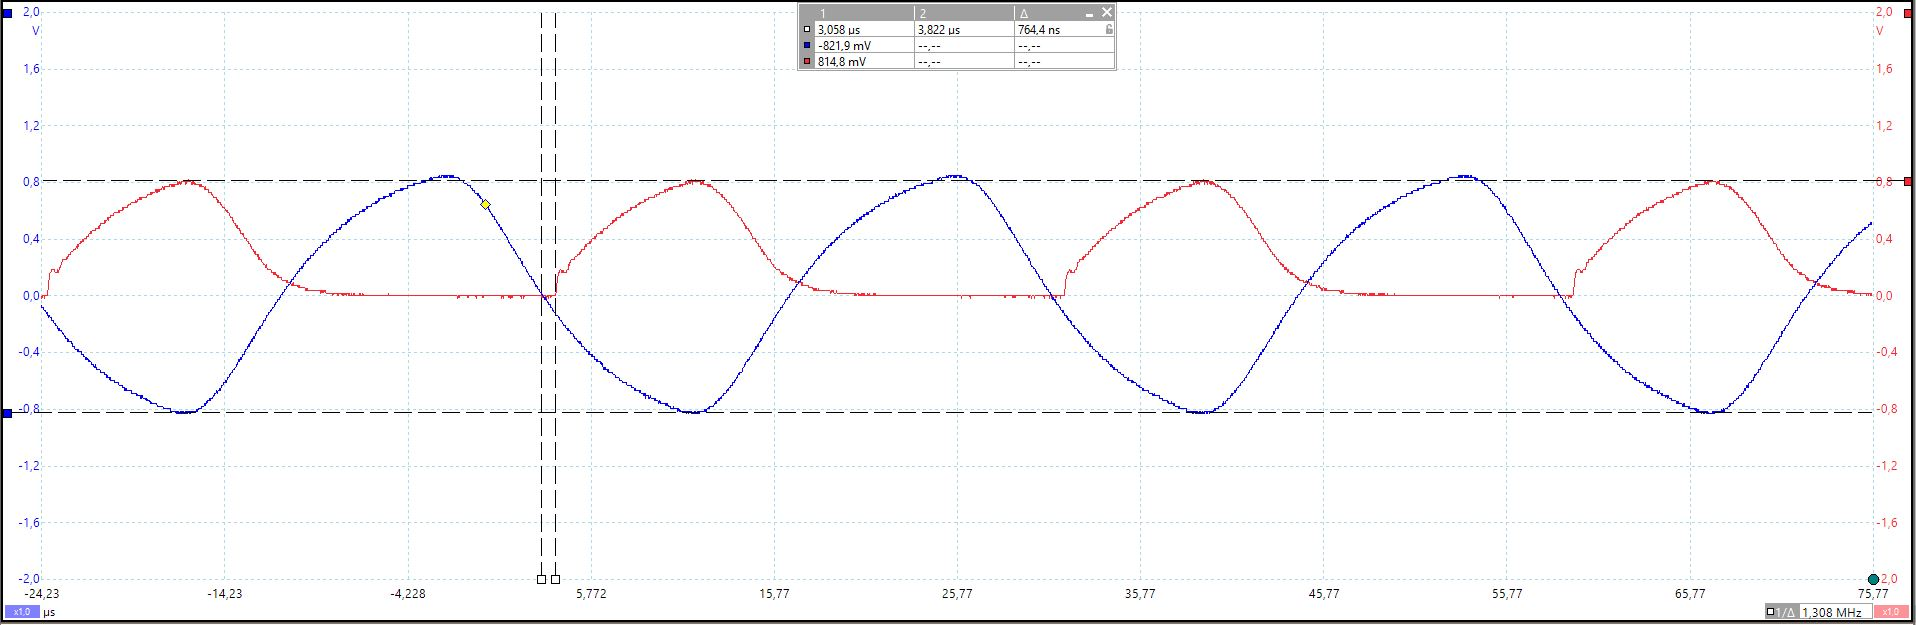
\includegraphics[width=\textwidth]{figures/results/rectification/36kHz.JPG}
	\captionof{figure}{Osciliscope output showing signal before and after rectification}
	\label{fig:precision_rectification}
\end{figure}

%%%%%%%%%%	DISCUSSION	%%%%%%%%%%
\textbf{Discussion}\\
The precision rectification stage operates as expected, the difference between the amplitude of the input signal and output signal during rectification is 7mV.

A 765nS cross-over delay can be observed, this is the time that elapses between the instant the input becomes negative and the instant the output starts to rise. This occurs because the op-amp requires some time to swing the output the combined forward voltage of the two diodes.
%%%%%%%%%%	/DISCUSSION	%%%%%%%%%%




%%%%%%%%%%%%%%%%%%%%%%%%%%%%%%%%%%%%%%%%%%%




\subsection{Goertzel Filter Performance}

\subsubsection{Simulated Frequency Response}
\label{sec:results_frequency_response}

\begin{figure}[H]
	\centering
	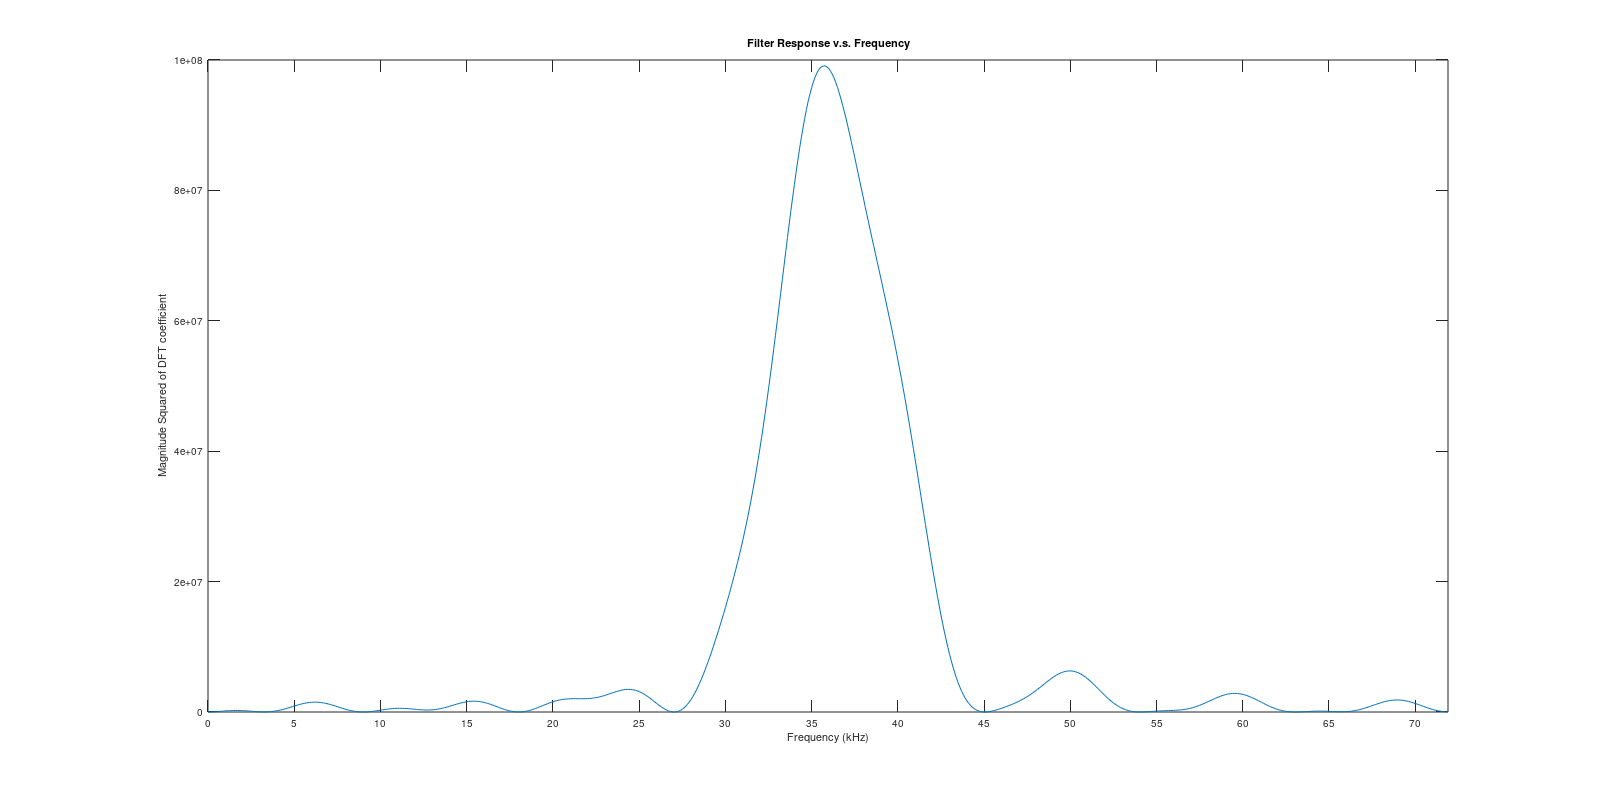
\includegraphics[width=\linewidth]{figures/results/goertzel_filter_simulation_wide.png}
	\caption{Expected Frequency Response - Goertzel Filter}
	\label{fig:goertzel_filter_response_simulated}
\end{figure}



%%%%%%%%%%	DISCUSSION	%%%%%%%%%%
\textbf{Discussion}\\
The simulation results in figure \ref{fig:goertzel_filter_response_simulated} reveal the familiar sinc like curve engrained in the frequency responses. More accurately the form of these curves is the $sinc^2(x)$ function which is expected because the filter returns the square of the magnitude.

From the plot, it can be seen that the filter is very sensitive to the magnitude of the sampled waveform. A decrease in amplitude by a factor of two results in a four-fold decrease in the amplitude of the filter's response.
%%%%%%%%%%	/DISCUSSION	%%%%%%%%%%




\subsubsection{Measured Frequency Response}

The following plot in figure \ref{fig:goertzel_filter_response_empirical} show the values returned by the Goertzel filter module and shows the expected frequency response curve.

\begin{figure}[H]
	\centering
	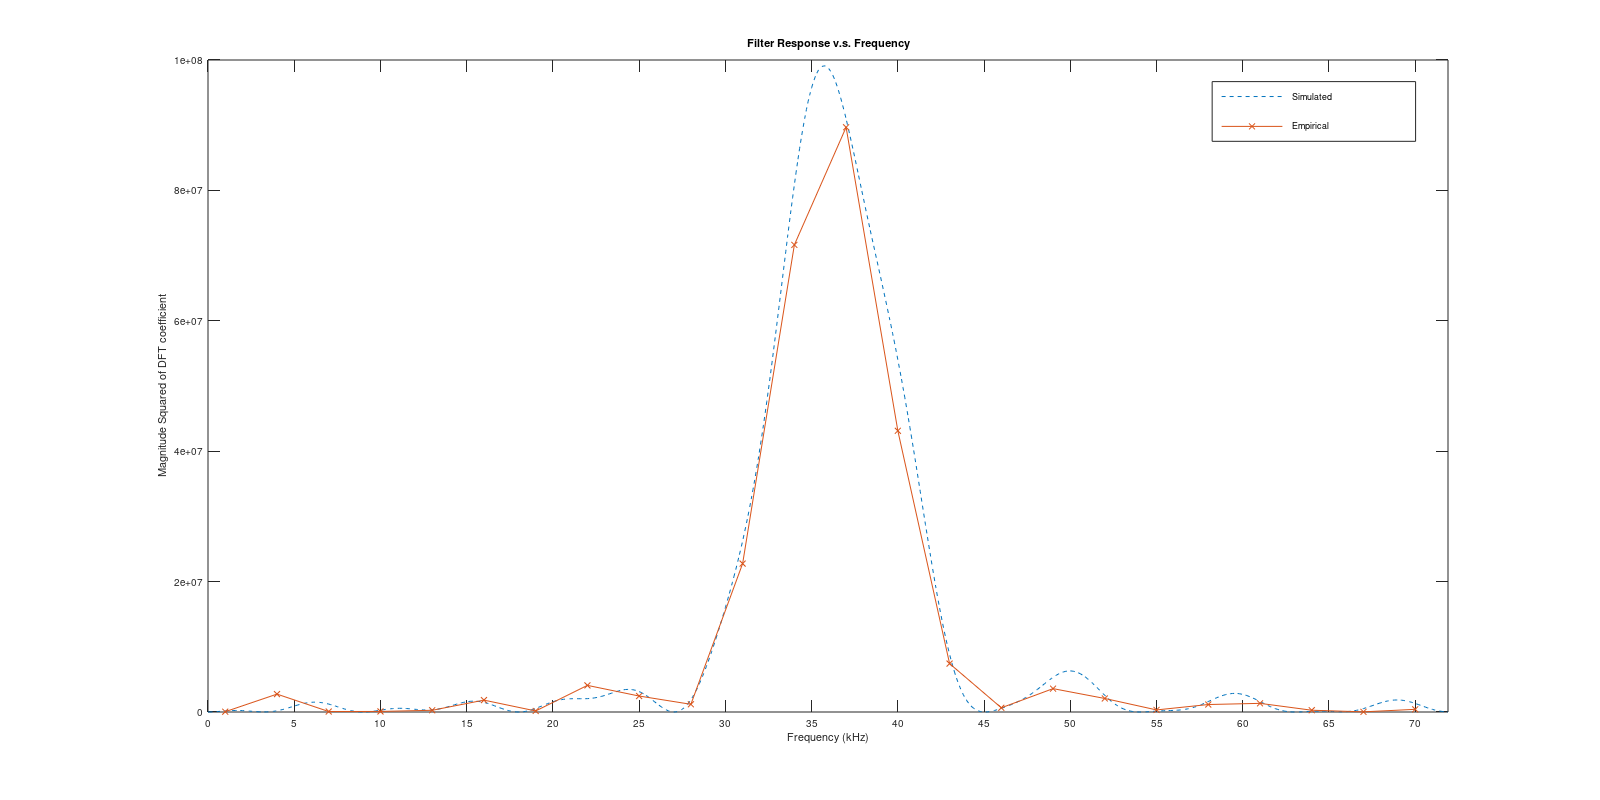
\includegraphics[width=\linewidth]{figures/results/goertzel_filter_empirical_wide.png}
	\caption{Measured Frequency Response - Optimized Goertzel Filter}
	\label{fig:goertzel_filter_response_empirical}
\end{figure}


%%%%%%%%%%	DISCUSSION	%%%%%%%%%%
\textbf{Discussion}\\
From these results, it is clear that the implemented algorithm is operating as expected. The small deviations from the expected response can be attributed to imperfections in the test signal and noise introduced by the ADC.
%%%%%%%%%%	/DISCUSSION	%%%%%%%%%%




\subsubsection{Trigger Conditions}

For a given waveform amplitude, table \ref{tbl:amplitude_voltage_trigger_pairs} lists the lower and upper-frequency bounds between which the tone decoder module outputs a high signal. These results were used to create the plot shown in figure \ref{tbl:amplitude_voltage_trigger_pairs}.

\begin{table}[H]
	\centering
	\begin{tabular}{ccc}
		\hline
		\begin{tabular}[c]{@{}c@{}}Amplitude\\ (mV)\end{tabular} & \begin{tabular}[c]{@{}c@{}}Trigger Frequency\\ Lower (kHz)\end{tabular} & \begin{tabular}[c]{@{}c@{}}Trigger Frequency\\ Upper (kHz)\end{tabular} \\ \hline
		297 & 35.12 & 36.79 \\ \hline
		300 & 34.7 & 37.23 \\ \hline
		350 & 32.74 & 39.27 \\ \hline
		400 & 31.86 & 40.16 \\ \hline
		450 & 31.29 & 40.78 \\ \hline
		500 & 30.86 & 41.2 \\ \hline
	\end{tabular}
	\captionof{table}{Amplitude-Voltage Boundry Pairs}
	\label{tbl:amplitude_voltage_trigger_pairs}
\end{table}

The green area in figure \ref{fig:goertzel_amplitude_frequency_pairs} represents the set of amplitude-frequency pairs, for amplitudes less than 500mV, which trigger the tone decoder.


\begin{figure}[H]
	\centering
	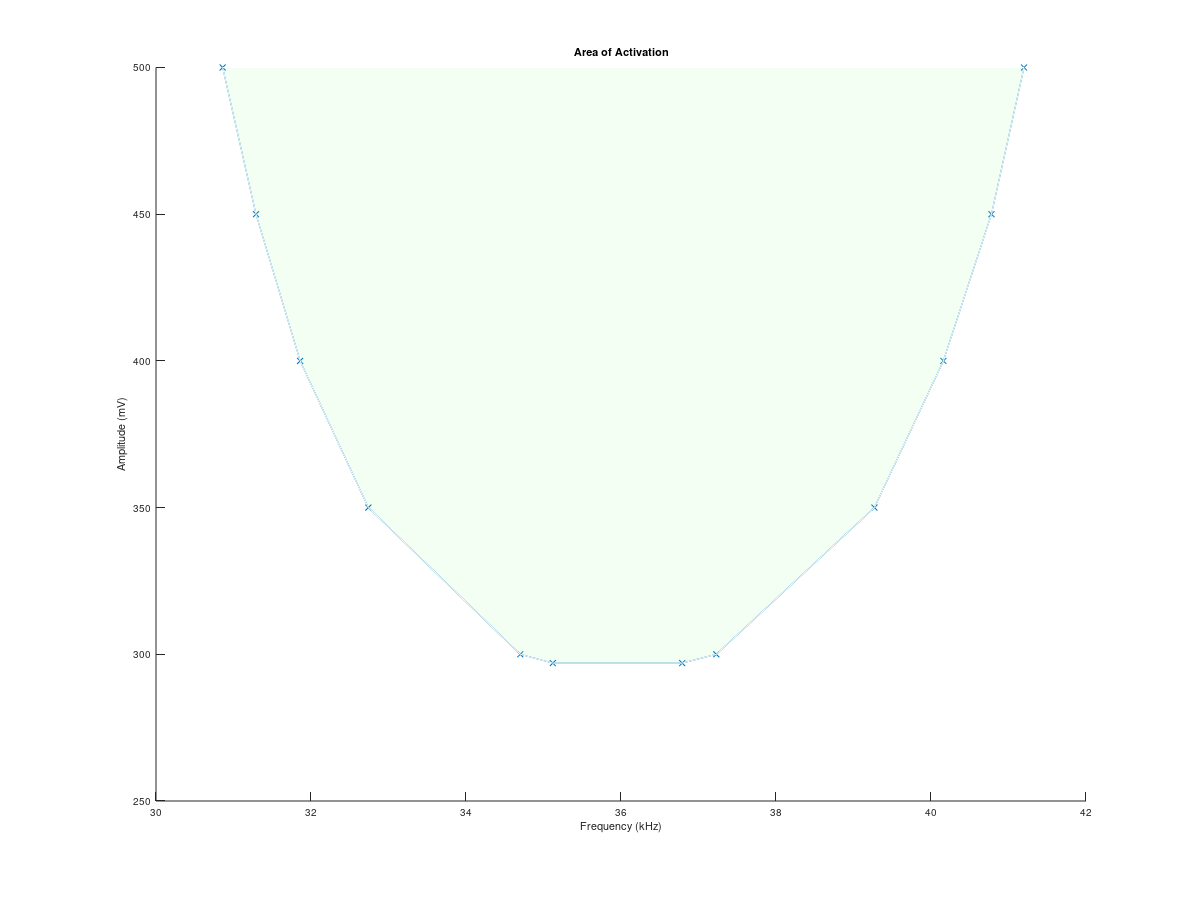
\includegraphics[width=.8\textwidth]{figures/results/goertzel_amplitude_frequency_pairs.png}
	\captionof{figure}{Area of Sensitivity Goertzel Filter}
	\label{fig:goertzel_amplitude_frequency_pairs}
\end{figure}




%%%%%%%%%%	DISCUSSION	%%%%%%%%%%
\textbf{Discussion}\\
The area of activation shows that for small input signals, the filter is not able to detect the presence of a carrier frequency. The filter could be made more sensitive to small signals by reducing the trigger value, however, this sufficiently broadens the trigger bandwidth. A more appropriate solution would be the inclusion of an automatic gain control stage to amplify small signals.
%%%%%%%%%%	/DISCUSSION	%%%%%%%%%%



%%%%%%%%%%%%%%%%%%%%%%%%%%%%%%%%%%%%%%%%%%%



%%%%%%%%%%%%%%%%%%%%%%%%%%%%%%%%%%%%%%%%%%%
%%%%%%%%%%%%%%%%%%%%%%%%%%%%%%%%%%%%%%%%%%%

%%%%%%%%%%%%%%%%%%%%%%%%%%%%%%%%%%%%%%%%%%%
%%%%%%%%%%%%%%%%%%%%%%%%%%%%%%%%%%%%%%%%%%%

\section{Software Evaluation}


\subsection{Goertzel Filter Benchmark}

Figure \ref{fig:goertzel_speed_scope_screenshot} shows the output traced by the oscilloscope during an iteration of this experiment. For both traces, a high logic level indicates the callback function is currently processing a portion of the circular buffer. The two traces distinguish between the different halves of the buffer.

For each iteration, the oscilloscope software was used to calculate the average processing time. The results are tabulated in table \ref{tbl:goertzel_speed_results}.

\begin{figure}[H]
	\centering
	\begin{minipage}{.45\textwidth}
		\centering
		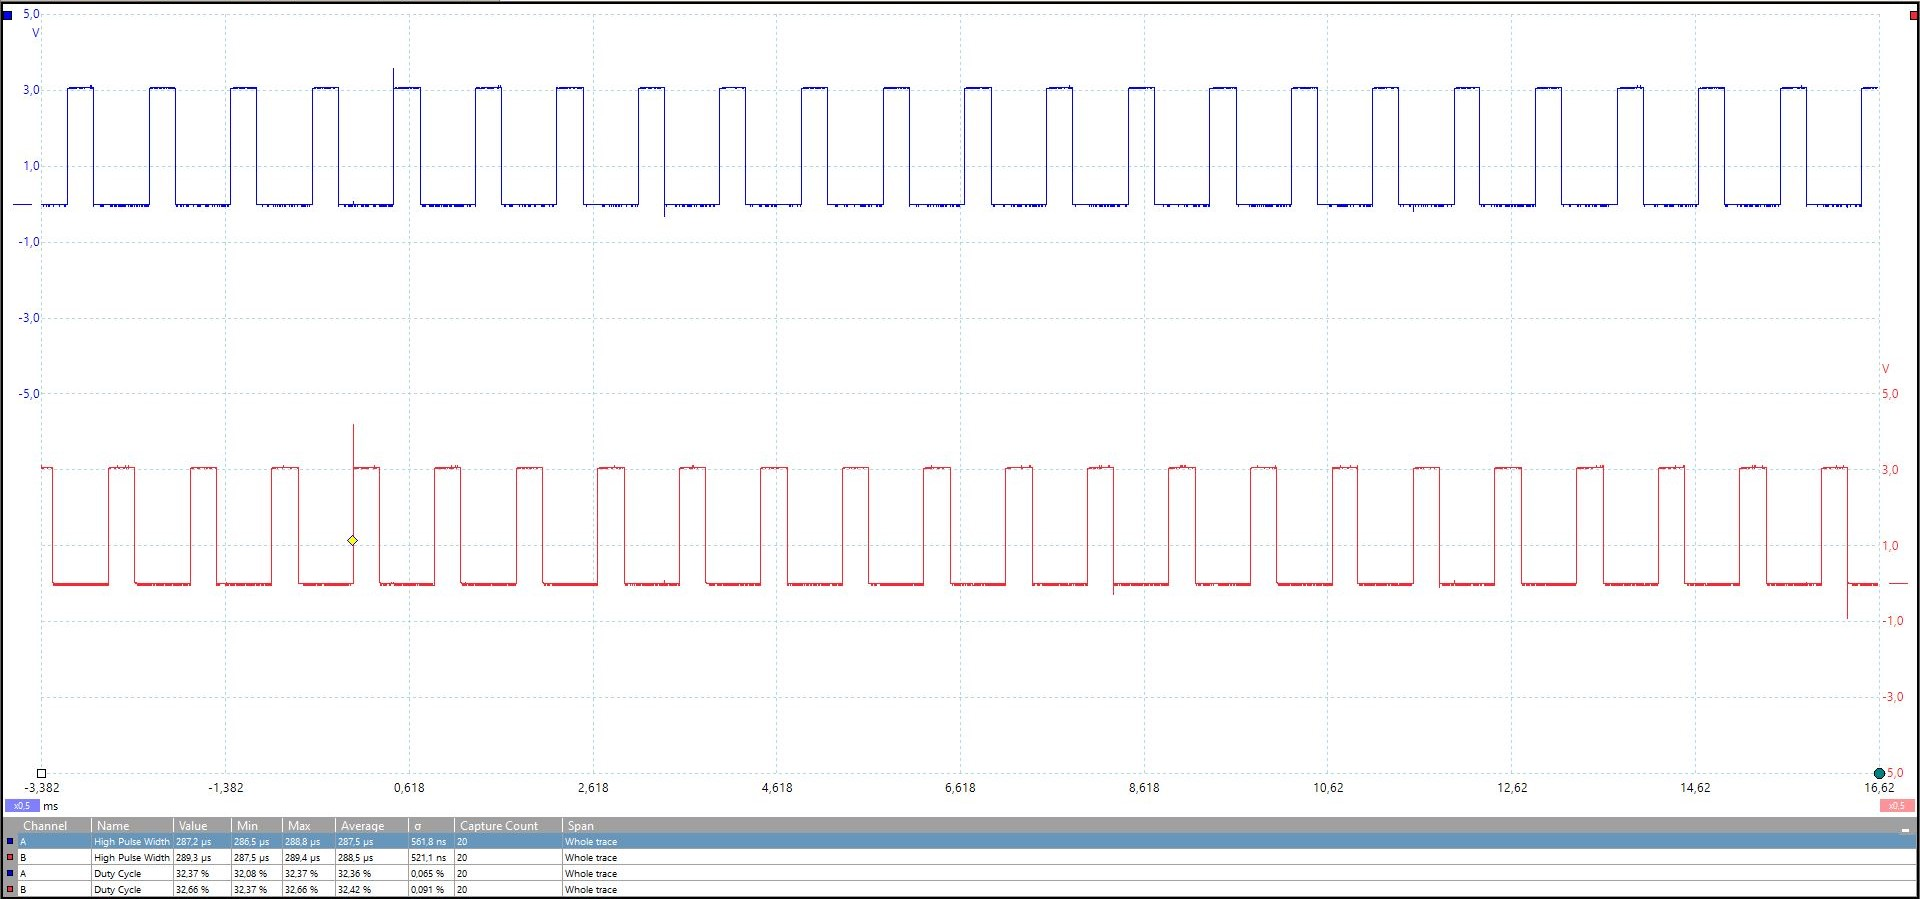
\includegraphics[width=0.9\linewidth]{figures/results/goertzel_filter_speed/16nu_crop.JPG}
		\captionof{figure}{Unoptimized Goertzel Algorithm with $N = 16$}
		\label{fig:goertzel_speed_scope_screenshot}
	\end{minipage}%
	\hspace{.05\textwidth}
	\begin{minipage}{.4\textwidth}
		\begin{table}[H]
			\begin{tabular}{ccc}
				\hline
				\textbf{N} & \textbf{\begin{tabular}[c]{@{}c@{}}Unoptimized\\ ($\mu S$)\end{tabular}} & \textbf{\begin{tabular}[c]{@{}c@{}}Optimized\\ ($\mu S$)\end{tabular}} \\ \hline
				4 & 96.46 & 61.15 \\ \hline
				8 & 160.3 & 98.35 \\ \hline
				16 & 287.5 & 171.9 \\ \hline
				32 & 547.2 & 323.9 \\ \hline
				64 & 1059 & 621.1
			\end{tabular}
			\captionof{table}{Compiled results for goertzel speed experiemnt}
			\label{tbl:goertzel_speed_results}
		\end{table}
	\end{minipage}
\end{figure}

Figure \ref{fig:goertzel_computation_plot} visualizes the results from table \ref{tbl:goertzel_speed_results} in a plot.

\begin{figure}[H]
	\centering
	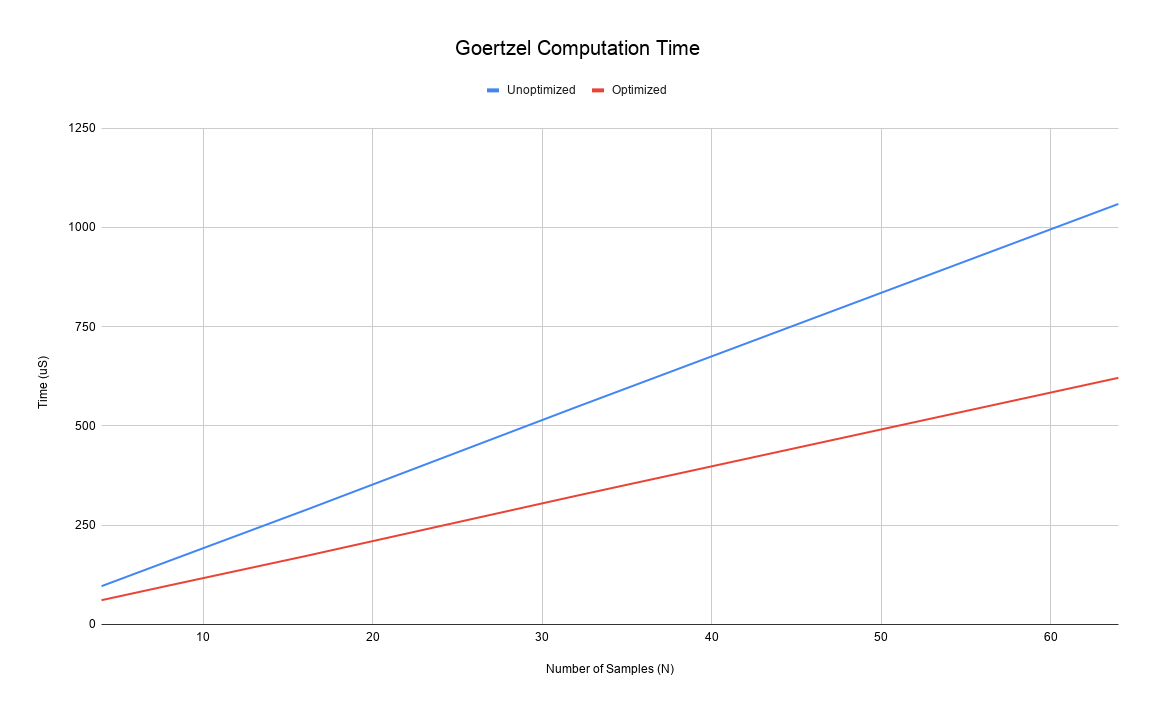
\includegraphics[width=\linewidth]{figures/results/goertzel_filter_speed/goertzel_computation_time.png}
	\captionof{figure}{Computation time versus the number of samples}
	\label{fig:goertzel_computation_plot}
\end{figure}


%%%%%%%%%%	DISCUSSION	%%%%%%%%%%
\textbf{Discussion}\\
Figure \ref{fig:goertzel_computation_plot} provides two important insights into the nature of the Goertzel algorithm.

The first observation may be found in the linearity of both plots, this confirms that both implementations of the algorithm have a time complexity of O(N) as noted in section \ref{sec:filter_optimization_design}. The essentially perfect linearity in the results makes it possible to predict timing requirements and make accurate theoretical predictions.

The gradient of the unoptimized curve is $16\mu S/sample$ and the gradient of the optimized curve is $9.3\mu S/sample$. The sampling rate used was $f_{sampling} \approx 144$kHz which translates to $T_{sampling} = 6.9\mu S/sample$. This indicates that even after optimizing the algorithm through the removal of unnecessary multiplications, the processor is still not fast enough to keep up with the rate of incoming samples.

The second observation is that the optimization has two performance implications. The first implication is a small but non-zero constant time saving, this comes by way of removing the two multiplications originally required to find the real and imaginary components of the k\textsubscript{th} DFT coefficient (see lines 18 and 19 of listing \ref{lst:goertzel_algorithm}). The second implication is a time difference which is directly proportional to the number of samples N, as indicated by the different gradients seen in figure \ref{fig:goertzel_computation_plot}.
%%%%%%%%%%	/DISCUSSION	%%%%%%%%%%


%%%%%%%%%%%%%%%%%%%%%%%%%%%%%%%%%%%%%%%%%%%



\subsection{Tagger MCU Performance}

\subsubsection{Manchester Encoding}
The oscilloscope trace in figure \ref{fig:manchester_sequence_141_decoded} shows the Manchester encoded waveform generated by the tagger, transmitting the number 141.

\begin{figure}[H]
	\centering
	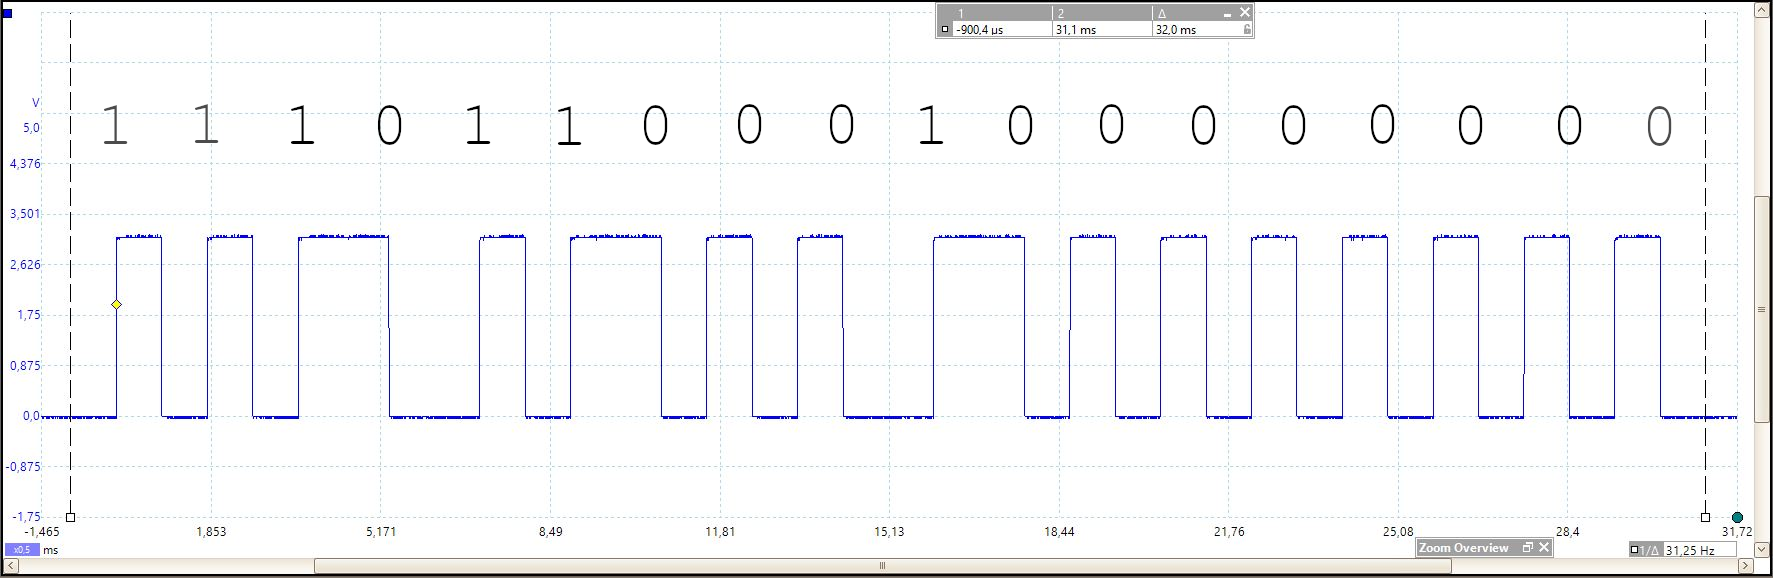
\includegraphics[width=.9\textwidth]{figures/results/manchester/manchester_sequence_141_decoded.png}
	\caption{Manchester Encoded Waveform}
	\label{fig:manchester_sequence_141_decoded}
\end{figure}

The bit period was measured to be 1.777ms, figure \ref{fig:delta_bit_period} in the appendix shows this measurement.


%%%%%%%%%%	DISCUSSION	%%%%%%%%%%
\textbf{Discussion}\\
Inspecting the decoded binary sequence (inserted above the waveform), the two start bits are seen, followed by the binary representation of the number 141 (in reverse). The 18\textsubscript{th} bit is a zero, which is the expected parity value for the data being transmitted.

The bit period of the waveform matched the expected value of 1.777ms, confirming the functionality of the module and demonstrating the high precision that may be achieved through the use of interrupts and timers.
%%%%%%%%%%	/DISCUSSION	%%%%%%%%%%



%%%%%%%%%%%%%%%%%%%%%%%%%%%%%%%%%%%%%%%%%%%



\subsection{Target MCU Performance}

\subsubsection{Processing Time}

\begin{figure}[H]
	\centering
	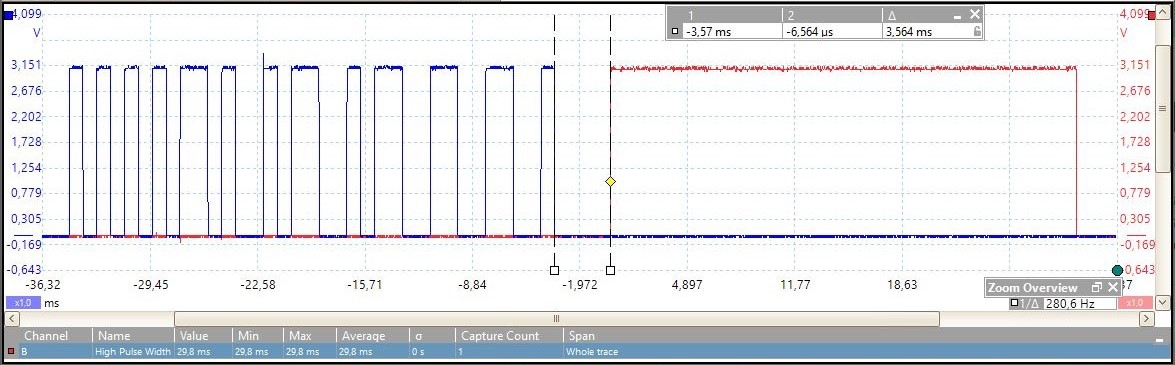
\includegraphics[width=.9\textwidth]{figures/results/receiver_software/arbitrary_11111_timing_test_crop_crop.JPG}
	\caption{Transmission of Decimal Number 11111}
	\label{fig:arbitrary_11111_timing_test}
\end{figure}

\begin{table}[H]
	\centering
	\begin{tabular}{cccc}
		\hline
		\textbf{\begin{tabular}[c]{@{}c@{}}15-Bit Data\\ (Decimal)\end{tabular}} & \textbf{Number of Edges} & \textbf{\begin{tabular}[c]{@{}c@{}}Timeout Delay\\ (ms)\end{tabular}} & \textbf{\begin{tabular}[c]{@{}c@{}}Processing Time\\ (ms)\end{tabular}} \\ \hline
		10922 & 20 & 3.56 & 29.7 \\ \hline
		11111 & 26 & 3.56 & 29.8 \\ \hline
		32767 & 36 & 3.56 & 29.9 \\ \hline
	\end{tabular}
\end{table}

Combining the timeout delay and processing time gives a maximum period of 33.46ms in the worst case, before a new message can be received.


%%%%%%%%%%	DISCUSSION	%%%%%%%%%%
\textbf{Discussion}\\
These results show that the number of edges in a typical transmission has a negligible effect on the total time taken to process the received data. Most of this processing time can be attributed to communication with the LCD.

The original RC-5 standard specifies a 114ms period between transmissions, this is significantly longer than necessary.

%%%%%%%%%%	/DISCUSSION	%%%%%%%%%%

\subsubsection{Error Handling}
Figure \ref{fig:transmission_too_fast} below shows a set of incoming transmissions (blue trace) that arrive faster than the MCU can process them. Any edges that occur while the MCU is processing a previous message (indicated by the red trace being high) are ignored.

\begin{figure}[H]
	\centering
	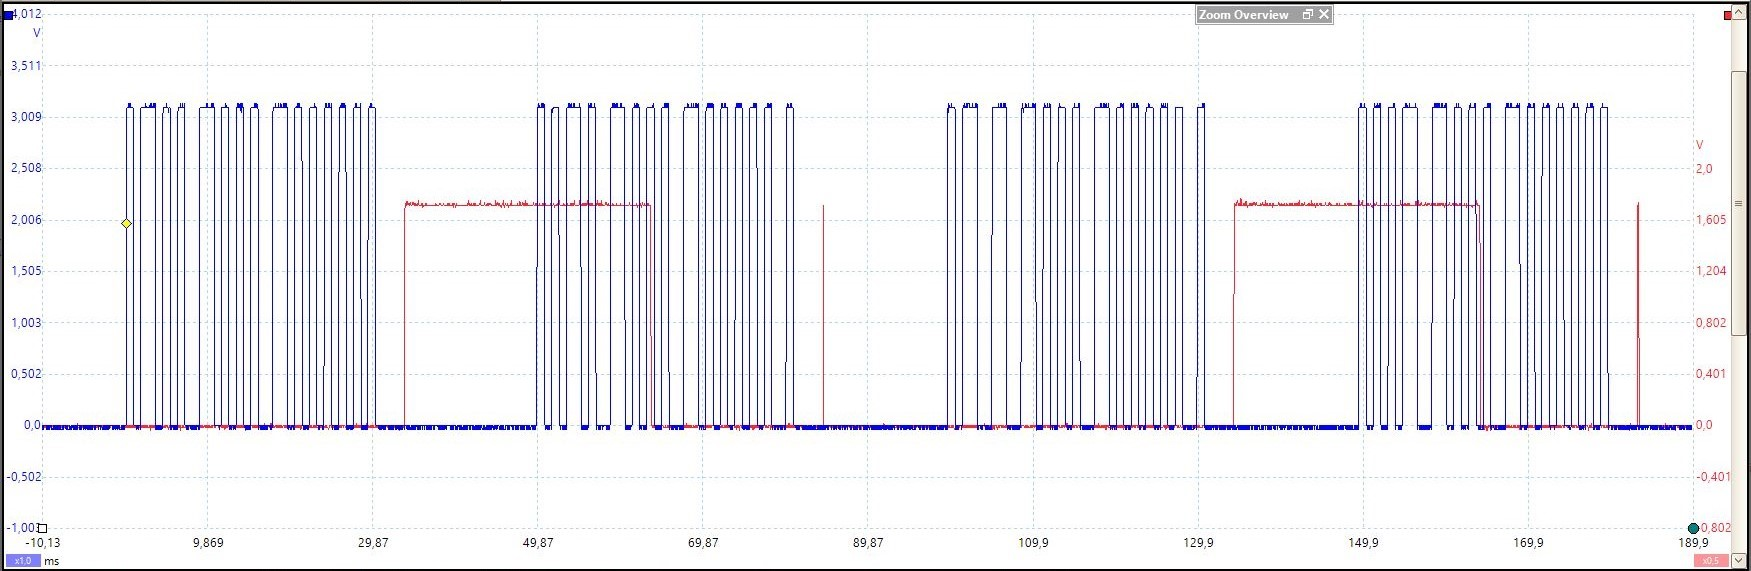
\includegraphics[width=.8\textwidth]{figures/results/receiver_software/transmission_too_fast_crop_crop.JPG}
	\caption{Incoming Transmission During Decoding}
	\label{fig:transmission_too_fast}
\end{figure}

Figure \ref{fig:transmission_too_many_edges} below shows an incoming stream of transmissions with no delay period separating them (blue trace). The time spent processing incoming transmissions is indicated by a high logic level on channel B (red trace).

\begin{figure}[H]
	\centering
	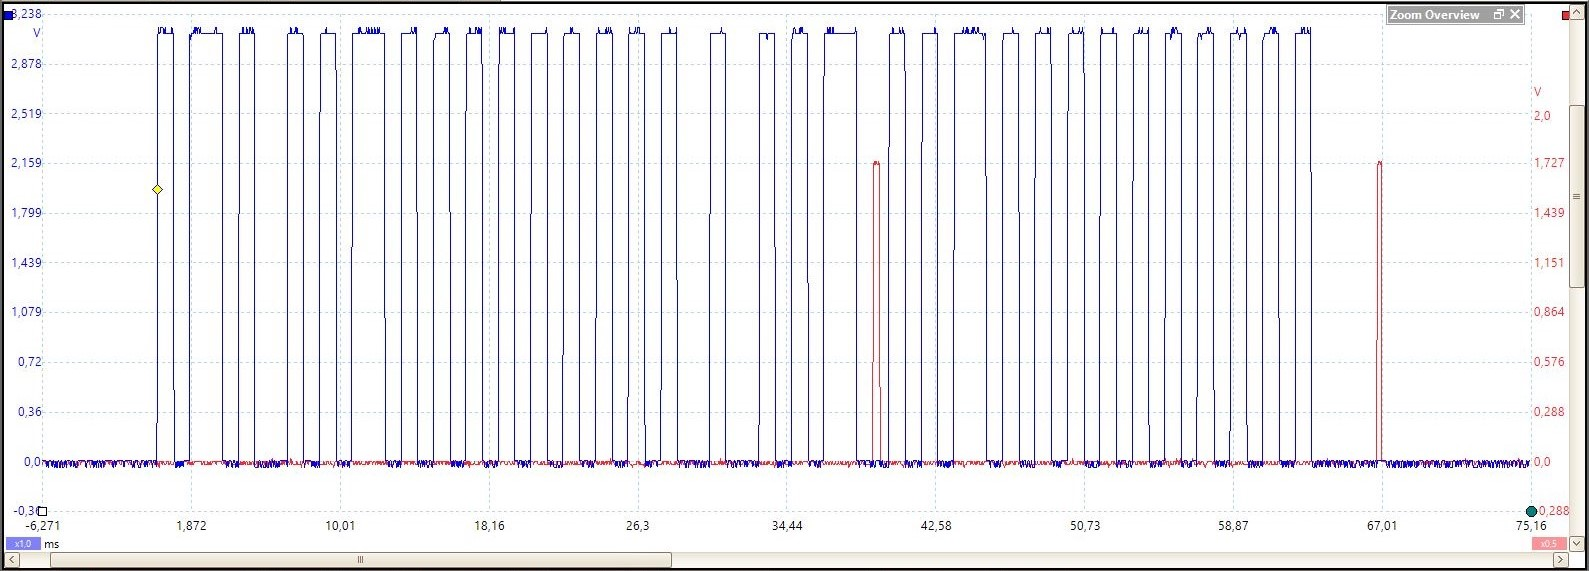
\includegraphics[width=.8\textwidth]{figures/results/receiver_software/transmission_too_many_edges_crop_crop.JPG}
	\caption{Continuous Transmission}
	\label{fig:transmission_too_many_edges}
\end{figure}

%%%%%%%%%%	DISCUSSION	%%%%%%%%%%
\textbf{Discussion}\\
%It seems that the LCD write function is the reason it takes so long to 'process', it's not that it is so much drastically longer because it's going through all the states.... but its too little too late to change that because soo many experiments used that code...
In the case of the two transmissions that arrived while the processor was busy, errors were detected and no further processing was performed. This is indicated by the short processing spike that occurs in each case (figure \ref{fig:transmission_too_fast}).

In the case of continuous transmission, the maximum number of edges were recorded. When this occurred the processor immediately attempted to decode the transmission. At the point when the number of decoded bits exceeded 18, the message was discarded and no further processing was performed (figure \ref{fig:transmission_too_many_edges}).

Both cases show that the error handling functionality is successful in the identification of errors.
%%%%%%%%%%	/DISCUSSION	%%%%%%%%%%




%%%%%%%%%%%%%%%%%%%%%%%%%%%%%%%%%%%%%%%%%%%


%%%%%%%%%%%%%%%%%%%%%%%%%%%%%%%%%%%%%%%%%%%
%%%%%%%%%%%%%%%%%%%%%%%%%%%%%%%%%%%%%%%%%%%

%%%%%%%%%%%%%%%%%%%%%%%%%%%%%%%%%%%%%%%%%%%
%%%%%%%%%%%%%%%%%%%%%%%%%%%%%%%%%%%%%%%%%%%

\section{System Range}

Table \ref{tbl:max_distances_system} below records the maximum range of the system under different ambient lighting conditions and records how that range changes as consequence of using the different detector modules.

\begin{table}[H]
	\centering
	\begin{tabular}{ccc}
		\hline
		Module & \begin{tabular}[c]{@{}c@{}}Maximum Distance\\ Dark Environment\\ (m)\end{tabular} & \begin{tabular}[c]{@{}c@{}}Maximum Distance\\ Bright Environment\\ (m)\end{tabular} \\ \hline
		Phototransistor & 17 & 36 \\ \hline
		Photodiode & 17.5 & SAT \\ \hline
		IR Receiver & 47 \textgreater{} & 47 \textgreater{} \\ \hline
	\end{tabular}
	\caption{Maximum Receiver Distances}
	\label{tbl:max_distances_system}
\end{table}

%%%%%%%%%%	DISCUSSION	%%%%%%%%%%
\textbf{Discussion}\\
The results show that the IR receiver module outperformed both the phototransistor and photodiode detector modules. The range of the IR receiver exceeded the length of the test environment.

The photodiode detector module saturated in the bright environment, this was as a consequence of the transimpedance amplifier design which only performed decoupling after the first amplification stage.

In the dark environment, both the phototransistor and photodiode modules achieved a similar range despite using different circuit designs to detect the incoming light.

The range of the phototransistor detector during the day was more than twice that of the range observed at night. This was contrary to expectations, it was assumed that the module would perform poorly in a bright environment due to the excessive ambient IR generated by the sun.
It might be possible that the ambient IR light caused the phototransistor to operate at a higher sensitivity, however, it is more plausible that environmental factors (for example a fine mist forming in the evening) caused the decrease in system range.

Both the photodiode and phototransistor modules were particularly sensitive to the strength of the IR beam. Adjusting the beam to be more than a couple of degrees off centre prevented the target system from detecting incoming transmissions. This is in contrast to the IR receiver module which was much less sensitive to beam intensity.

The following screenshots present further observations that were made while testing the system range.
%%%%%%%%%%	/DISCUSSION	%%%%%%%%%%


\subsubsection{Photodiode Observations}

\begin{figure}[H]
	\centering
	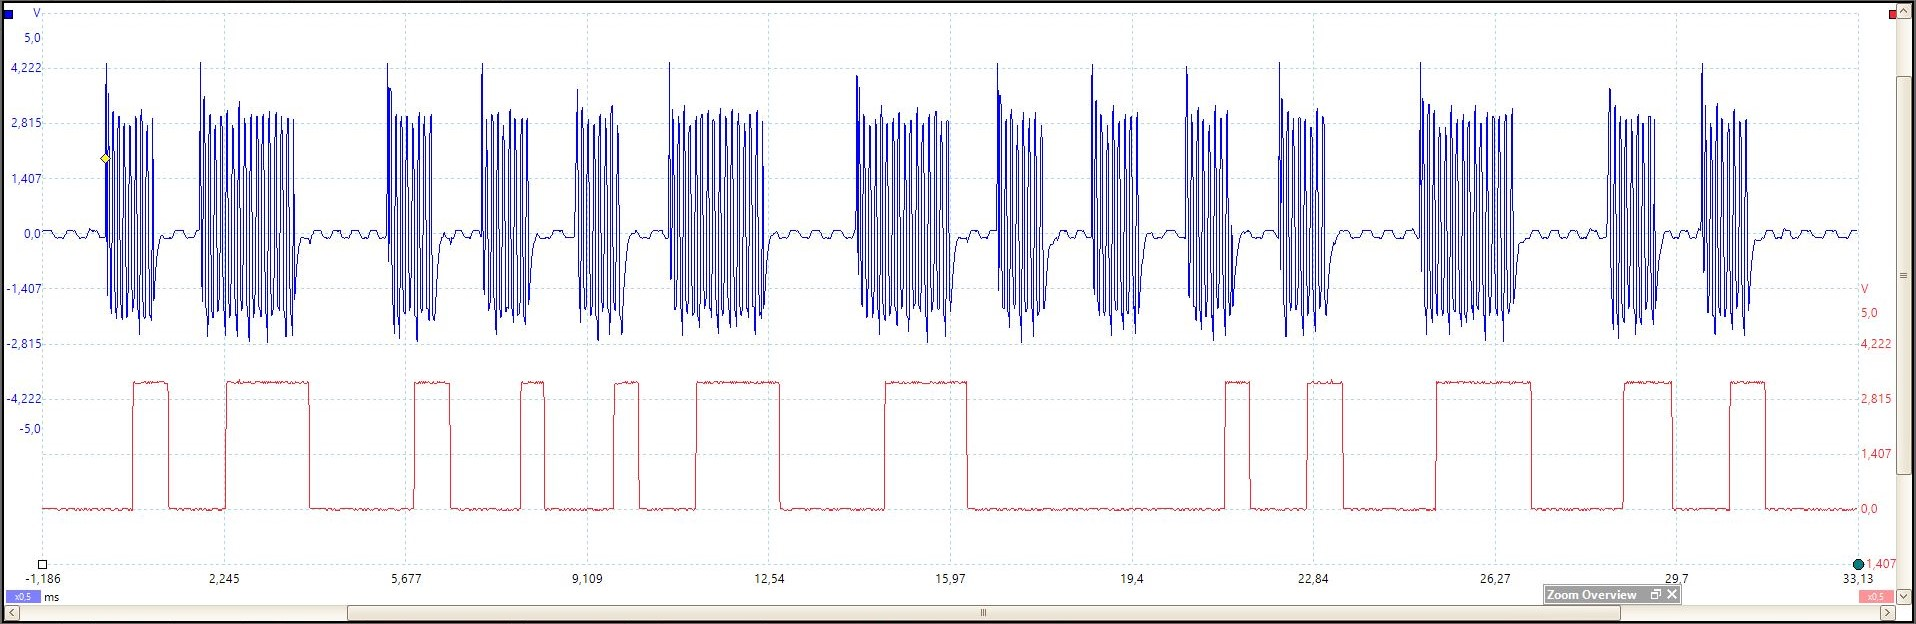
\includegraphics[width=.9\textwidth]{figures/results/drak_system_test/photodiode1750cm_missed_bits.jpg}
	\caption{Undetected bits in a dark environment at a range of 17.5m}
	\label{fig:photodiode_bit_error}
\end{figure}


\begin{figure}[H]
	\centering
	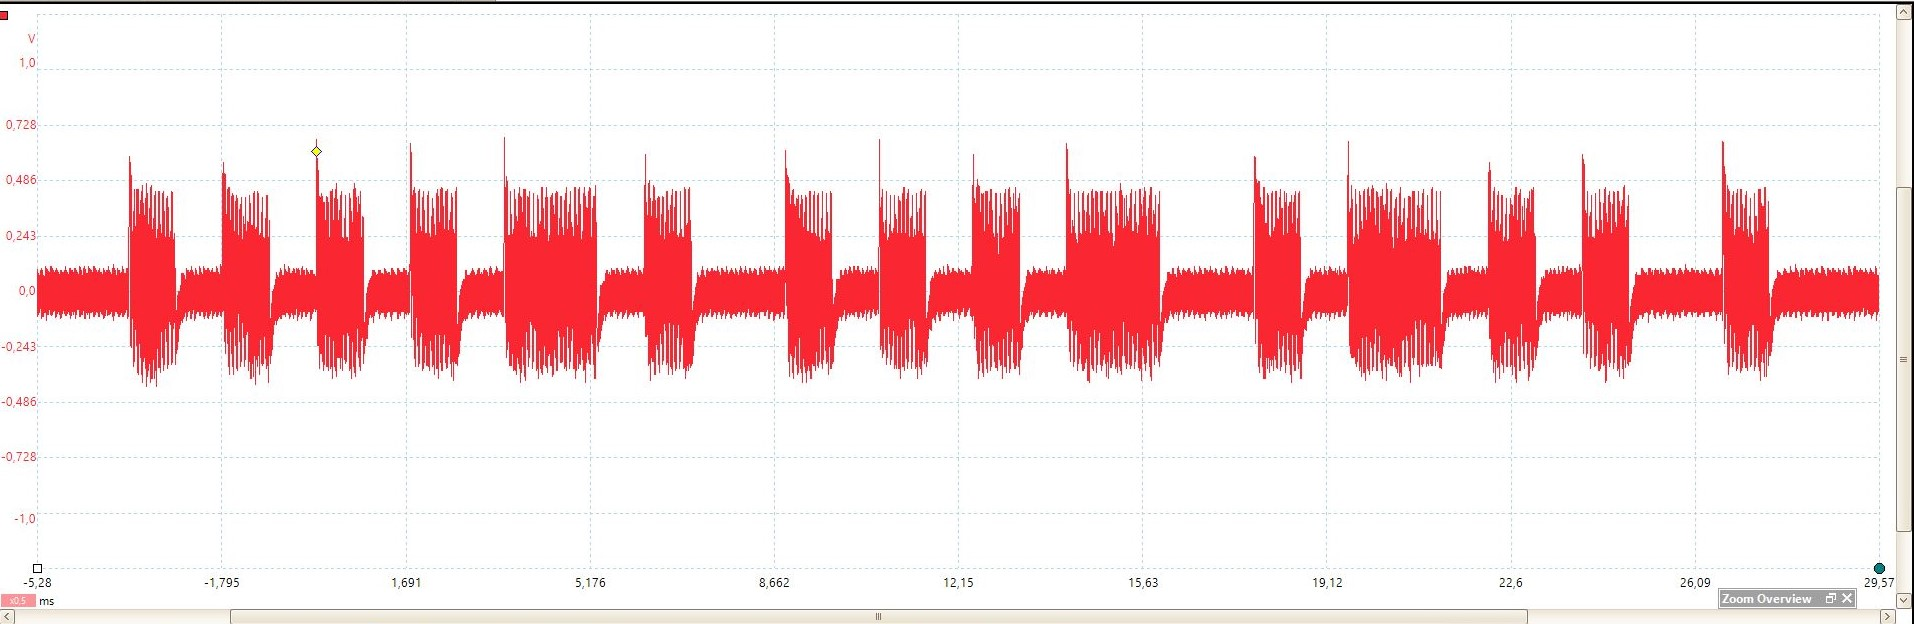
\includegraphics[width=.9\textwidth]{figures/results/drak_system_test/photodiode4770cm.jpg}
	\caption{Photodiode detector module's output in a dark environment at a range of 47m}
	\label{fig:photodiode_range_4770cm}
\end{figure}

%%%%%%%%%%	DISCUSSION	%%%%%%%%%%
Figure \ref{fig:photodiode_bit_error} shows the waveform at the input to the signal conditioning module (blue trace). Despite an exceptionally high signal to noise ration, the tone decoder fails to detect two modulation periods because the magnitude of the incoming signal is not great enough. The inability to adjust the gain of the waveform prior to the Goertzel filter is the biggest short-coming of the receiver system.  This problem can be solved through the use of an automatic gain control.

The potential for improvement is highlighted in figure \ref{fig:photodiode_range_4770cm} which shows the input to the signal conditioning module at a distance of 47m. Once again, despite the small signal amplitude there is a clear distinction between the modulating light signal and noise floor.
%%%%%%%%%%	/DISCUSSION	%%%%%%%%%%


\subsubsection{Phototransistor Observations}

\begin{figure}[H]
	\centering
	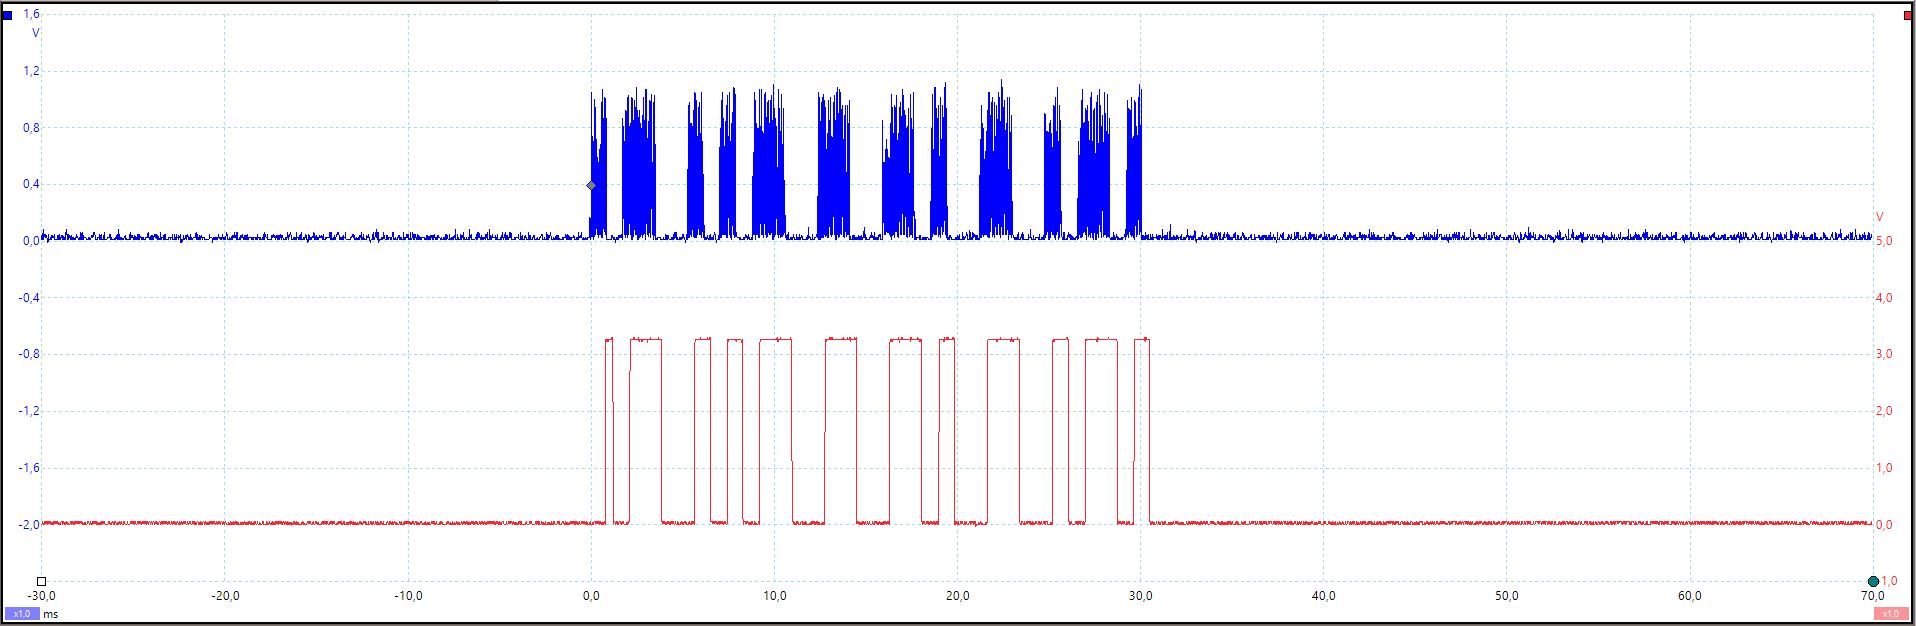
\includegraphics[width=.9\textwidth]{figures/results/system_test/36m_phototranaistoroutput.JPG}
	\caption{Phototransistor Detector in a bright environment at a range of 36m}
	\label{fig:phototransistor1}
\end{figure}


%%%%%%%%%%	DISCUSSION	%%%%%%%%%%
Figure \ref{fig:phototransistor1} above shows the input to the tone decoder (blue trace) and the output of the tone decoder module (red trace) at the maximum range for the phototransistor receiver in a bright environment. Once again, the signal to noise ratio is very high, even at a distance of 36m.
%%%%%%%%%%	/DISCUSSION	%%%%%%%%%%


\subsubsection{IR Receiver Observations}

\begin{figure}[H]
	\centering
	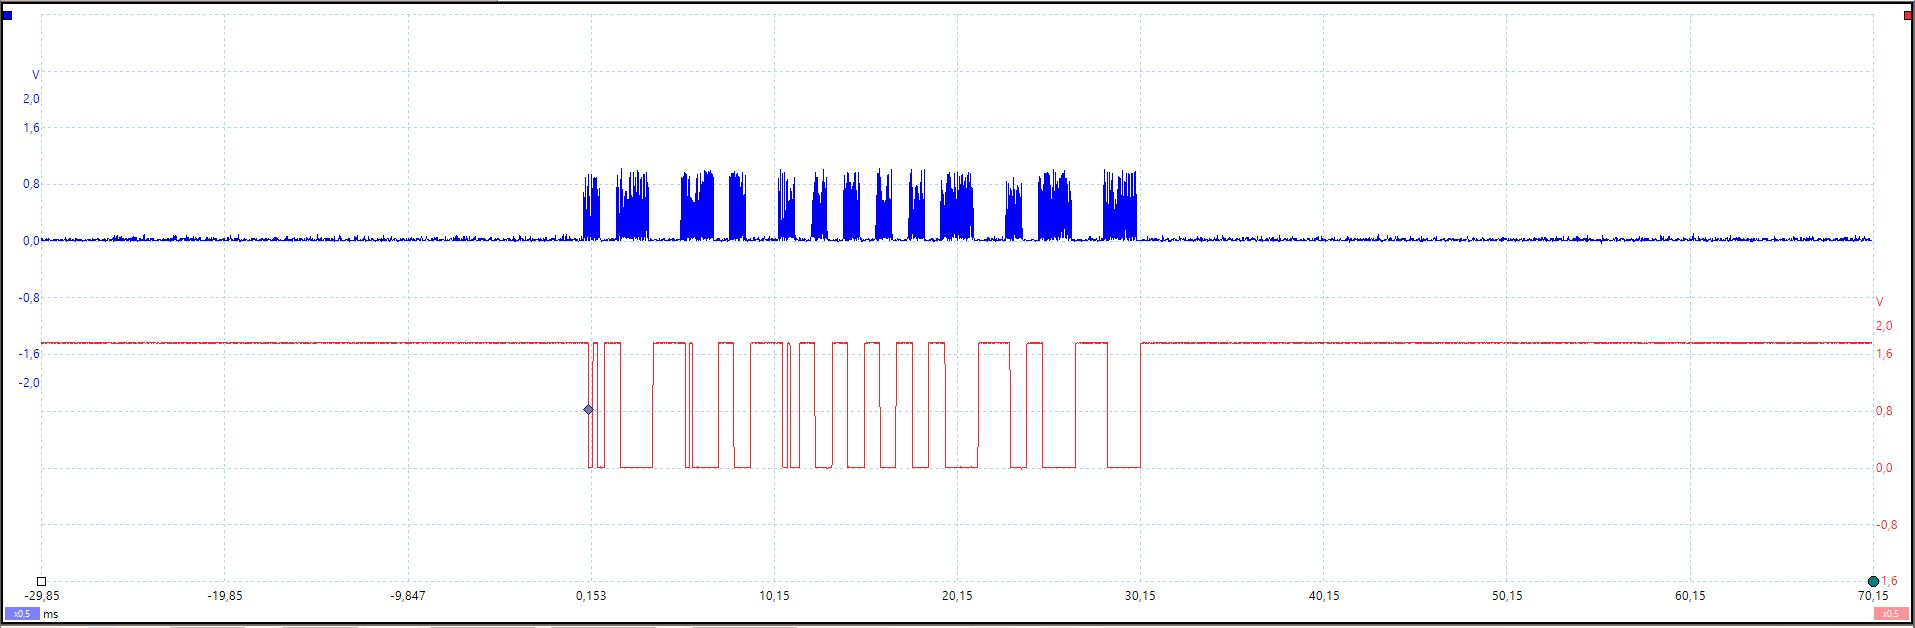
\includegraphics[width=.9\textwidth]{figures/results/system_test/36m_phototranaistoroutput_vs_ir_receiver.JPG}
	\caption{Output of the IR receiver and the conditioned output of the phototransistor detector}
	\label{fig:36m_phototranaistoroutput_vs_receiveroutput}
\end{figure}

%%%%%%%%%%	DISCUSSION	%%%%%%%%%%
While testing the IR receiver in the bright environment blips could be observed. These are shown in figure \ref{fig:36m_phototranaistoroutput_vs_receiveroutput}, which shows the output of the IR receiver (red trace) and the output of the signal conditioning module (blue trace) which is coupled to the phototransistor detector. These blips were only observed while the IR receiver was centred on the incoming beam and would cease to occur if the receiver was moved slightly off-centre.

These blips produced errors in the decoded bit-stream by causing the target MCU to register invalid edges. The cause of these blips is unknown, they are possibly an artefact of the automatic gain control stage.
%%%%%%%%%%	/DISCUSSION	%%%%%%%%%%

%%%%%%%%%%%%%%%%%%%%%%%%%%%%%%%%%%%%%%%%%%%
%%%%%%%%%%%%%%%%%%%%%%%%%%%%%%%%%%%%%%%%%%%